%!TEX root = ../thesis.tex
%*******************************************************************************
%****************************** Second Chapter *********************************
%*******************************************************************************

\chapter{Results}
\label{sec:res}

This chapter summarizes the results of the measurement of the \ttbar production cross section at a center of mass energy of $\sqrt{s} = 13 \; \TeV$.
Before describing the main result in Section \ref{sec:results_main}, the results for  previous measurements with different data sets are shown
in Section \ref{sec:res_prev}. The first cross section measurement of the \ttbar cross section at $\sqrt{s}= 13 \; \TeV$ was measured with a small dataset using an integrated luminosity of $\lumi_{\mathrm{int}}= 42 \pbinv$ 
of data (see Section \ref{sec:res_ea}). After confirming the Standard Model expectation in this early measurement, a more precise measurent was performed with the full dataset taken in 2015 (see Section \ref{sec:res_2015}).
These two previous measurements illustrate the increase in precision for \ttbar cross section measurements at $\sqrt{s} = 13 \; \TeV$.

The description of the main result starts by illustrating the result of the template fit with the fitted distributions in Section \ref{sec:results_templates}.
A breakdown of the systematic uncertainties, including the fit results for relevant nuisance parameters, is given in Section \ref{sec:results_uncert}.

The measured \ttbar production cross section is compared to the theory prediction as well as to results from other experiments in Section \ref{sec:results_comp}.

The top quark pole mass is extracted in Section \ref{sec:res_mass}, based on the main result for the measurement of the \ttbar production cross section.

The effect of adding events from the single muon channel to the fit is discussed in Section \ref{sec:res_semi}.


\section{Results with the 2015 data sets}
\label{sec:res_prev}

Both results for the \ttbar cross section in this section are measured with data taken in 2015 by the CMS detector.
The measurements use the same basic method as the main result with the key difference of using only the \emu decay.
They were both used to cross check the main results in publications by the CMS collaboration \cite{Khachatryan:2015uqb,Khachatryan:2016kzg}.

\subsection{First measurement of the top pair production cross section at 13 TeV}
\label{sec:res_ea}

The first measurement of the \ttbar production cross section at $\sqrt{s}= 13 \TeV$ used $\lumi_{\mathrm{int}}= 42 \pbinv$ taken early in during the 2015 LHC run.
It is aimed at discovering possible deviations from the Standard Model at a new collision energy.
The analysis strategy is very similar to the one described in Section \ref{sec:xsec} with a few differences: 

\begin{itemize}
\item In order to reduce the contamination from background processes, only events in the \emu channel are selected for the measurement.
\item Due to the statistics in data, the event yields are chosen as templates for the fit instead of kinematic distributions of jets (see Figures \ref{fig:xsec_emu_inputdistr} for the templates used in the main result).
\item A very simple strategy is used to select events at the trigger level, since the low amount of available data makes any more comprehensive treatment difficult.
\item Systematic uncertainties are in general less detailed, especially the uncertainties on the theoretical predictions. Due to large uncertainties
from data statistics and luminosity, a more detailed study of further systematic uncertainties can be neglected.
\end{itemize}

Using the template fit, the \ttbar cross section in the full phase space is measured as:

\begin{equation}
\sttbar = 778 \pm  54 ({\rm stat}) \pm 61 ({\rm syst}) \pm 76 ({\rm lumi}) \pb.
\end{equation}

The uncertainty on the luminosity is the highest single uncertainty, but the statistical uncertainty and the uncertainty from the other systematic sources are of the same order of magnitude.
The breakdown of the systematic uncertainties is shown in Table \ref{tab:res_ea}.

\begin{table}[htbp!]
\begin{center}
\caption{Results of the first measurement of the \ttbar cross section at $\sqrt{s}= 13 \TeV$. The systematic uncertainties are broken down by their sources.  }
\label{tab:res_ea}
\begin{tabular}{ l|c}
 \hline
Name  & Contribution [\%] \\ \hline
Trigger    & $\pm^{4.0}_{2.9}$ \\
Lepton ID/isolation    & $\pm^{3.4}_{2.4}$ \\
Lepton energy scale    & $\mp^{0.2}_{0.1}$ \\
Jet energy scale    & $\pm^{2.7}_{2.1}$ \\
Jet energy resolution    & $\mp^{0.1}_{0.0}$ \\
B-tag    & $\pm^{0.8}_{0.7}$ \\
Mistag    & $\mp^{0.2}_{0.2}$ \\
Pile-up    & $\pm^{0.7}_{0.6}$ \\
NLO generator    & $\mp^{0.1}_{0.0}$ \\
$Q^{2}$ scale    & $\mp^{0.1}_{0.0}$ \\
PDF    & $\pm^{1.9}_{1.5}$ \\
DY background    & $\pm^{6.3}_{4.4}$ \\
Single top background   & $\mp^{1.5}_{1.5}$ \\
Diboson background    & $\pm^{3.5}_{2.4}$ \\
$t\bar{t}$ background    & $\mp^{0.3}_{0.3}$ \\
W+jets background    & $\pm^{0.4}_{0.3}$ \\
Luminosity    & $\pm^{11.1}_{8.4}$ \\
Stat    & $\mp{6.9}$ \\
Total vis    & $\pm^{15.6}_{12.9}$ \\ \hline
$\sigma_{t\bar{t}}$(13 TeV) vis    & 12.5 pb \\ \hline
$Q^{2}$ scale (extr)    & $\mp^{0.3}_{0.0}$ \\
PDF (extr)    & $\pm^{1.6}_{1.1}$ \\ \hline
Total    & $\pm^{15.6}_{13.0}$ \\ \hline
$\sigma_{t\bar{t}}$(13 TeV)    & 778 pb \\ \hline \hline
\end{tabular}
\end{center}
\end{table}

The total uncertainty of the measurement is dominated by experimental uncertainties. The contribution from theoretical uncertainties is negligible.
Besides the uncertainty on the luminosity the largest uncertainties come from the backgrounds, the determination of trigger, lepton efficiencies and jet energy scales.
The chosen templates for the fit show little discrimination between signal and background, leading to large contributions from the background uncertainties.
Similarly, there is little sensitivity for the jet energy scale in the templates, which limits the constraining power of the fit.

The high contribution from the trigger efficiency uncertainty shows the importance of maximising the trigger efficiencies and minimising their uncertainties.
This is the main motivation for the detailed trigger studies described in Section \ref{sec:Trigger}. 

\subsection{Measurement of the top quark pair production cross section with the 2015 data set}
\label{sec:res_2015}

This measurement of the \ttbar production cross section at $\sqrt{s}=13\TeV$ uses the full 2015 dataset taken by CMS with a luminosity of $\lumi_{\mathrm{int}}= 2.2 \fbinv$.
It should confirm the previous measurement (see Section \ref{sec:res_ea}) and allow a more precise comparison with theoretical predictions.
The analysis strategy is again very similar to the strategy for the main result described in Section \ref{sec:res_ea} with the following differences:

\begin{itemize}
\item Only events in the \emu channel are used.
\item The trigger selection is now similar to the one described in Section \ref{sec:TriggerSel}, but no detailed study on the systematic uncertainty on the trigger efficiency measurement is made (compare to Section \ref{sec:TriggerComp}).
\item The determination of theoretical systematic uncertainties uses a simpler method when compared to the main result.
\end{itemize}

With the template fit the \ttbar cross section measured to be:

\begin{equation}
\sttbar = 793 \pm  7 ({\rm stat}) \pm 27 ({\rm syst}) \pm 21 ({\rm lumi}) \pb .
\end{equation}

Compared to the analysis with early 2015 data, the uncertainty is reduced significantly. The decrease in statistical uncertainty reflects the larger dataset. The luminosity was determined with a higher precision, leading to a lower
uncertainty on the \ttbar cross section \cite{CMS-PAS-LUM-15-001}. The systematic uncertainties are detailed in Table \ref{tab:res_2015ana}.

\begin{table}[htbp!]
\begin{center}
\caption{Results of the \ttbar cross section at $\sqrt{s}= 13 \TeV$ with the full 2015 dataset. The systematic uncertainties are broken down by their sources. The uncertainty from the luminosity is externalized from the fit
and not included in the table.  }
\label{tab:res_2015ana}
\begin{tabular}{ l | c }
 \hline
Name  & Contribution [\%] \\ \hline
Trigger & ${1.3}$ \\
Lepton ID/isolation & ${1.4}$ \\
Lepton energy scale & ${0.5}$ \\
Jet energy scale & ${1.2}$ \\
Jet energy resolution  & ${0.1}$ \\
B-tag & ${0.3}$ \\
Mistag & ${0.1}$ \\
Pile-up & ${0.3}$ \\
NLO generator & ${0.2}$ \\
$Q^{2}$ scale  & ${0.5}$ \\
PDF & ${1.7}$ \\
Parton Shower & ${0.4}$ \\
BG\_tW/bar{t}W & ${1.5}$ \\
DY background & ${0.5}$ \\
Diboson background  & ${0.2}$ \\
$t\bar{t}$ background & ${0.3}$ \\
W+jets background & ${0.6}$ \\
Stat & ${0.9}$ \\
Total vis & ${3.2}$ \\ \hline
$\sigma_{t\bar{t}}$(13 TeV) vis & 12.73 pb \\ \hline
$Q^{2}$ scale (extr) & $\mp^{0.5}_{0.1}$ \\
PDF (extr) & $\pm^{1.0}_{1.7}$ \\ \hline
Total & $\mp^{3.5}_{3.3}$ \\ \hline
$\sigma_{t\bar{t}}$(13 TeV) & 793 pb \\ \hline \hline
\end{tabular}
\end{center}
\end{table}

Here, the main systematic uncertainties are the uncertainty on the PDF, the single top background, and the trigger and lepton efficiency uncertainties.
The uncertainty from the PDF is hard to constrain in the fit itself, but the main result uses an updated PDF set with lower uncertainties.
Similarly, the single top process is very hard to distinguish from the \ttbar signal. It has the same final state and very similar kinematic behaviour, consequently this uncertainty
is mostly irreducible.

The uncertainty on the trigger efficiency measurement again motivated the studies to reduce the systematic uncertainty on the efficiency measurement.
In order to reduce the uncertainties from the lepton efficiencies the same flavor channels are added to the measurement. Measuring the cross section
simultaneously in all three decay channels at least allows constraining the larger of the two lepton uncertainties as explained in Section \ref{sec:xsec_templates}.


\section{Measurement of the top quark pair production cross section with the 2016 data set}
\label{sec:results_main}

As described in Chapter \ref{sec:xsec}, the \ttbar production cross section is measured using a template fit.
The cross section is first measured in the visible phase space requiring a dileptonic decay with the two leptons meeting the requirements of $\pt (lead) > 25 \GeV, \pt (sublead) > 20\GeV$, $\abs{\eta} < 2.4$ 
and $\mll > 20 \GeV$ .
The result for the visible cross section is:

\begin{eqnarray*}
\sttvis & = & \resultxsecvismain. 
\end{eqnarray*}

The cross section is then extrapolated to the full phase space, resulting in:

 \begin{eqnarray*}
\sttbar & = & \resultxsecmain.
\end{eqnarray*}

These results are more precise than the two results presented above, showing the improvement of the measurement.
They are also consistent within their uncertainties.

\subsection{Post-fit template distribution}
\label{sec:results_templates}

The results of the measurement of the \ttbar cross section can be applied to the distributions used in the fit, including the fitted values for the
nuisance parameters and their constraints. The nuisance parameters are applied to the templates following the interpolation described in Section \ref{sec:xsec_stat}.
All nuisance parameters are considered including those related to the normalization of the background templates.

The resulting distributions are shown in Figures \ref{fig:lh_emu_postfitdistr8}, \ref{fig:lh_mumu_postfitdistr8} and \ref{fig:lh_ee_postfitdistr8}, with the background processes
being merged into one contribution.




\begin{figure}[htbp!]
  \begin{center}
    \resizebox{0.32 \textwidth}{!}{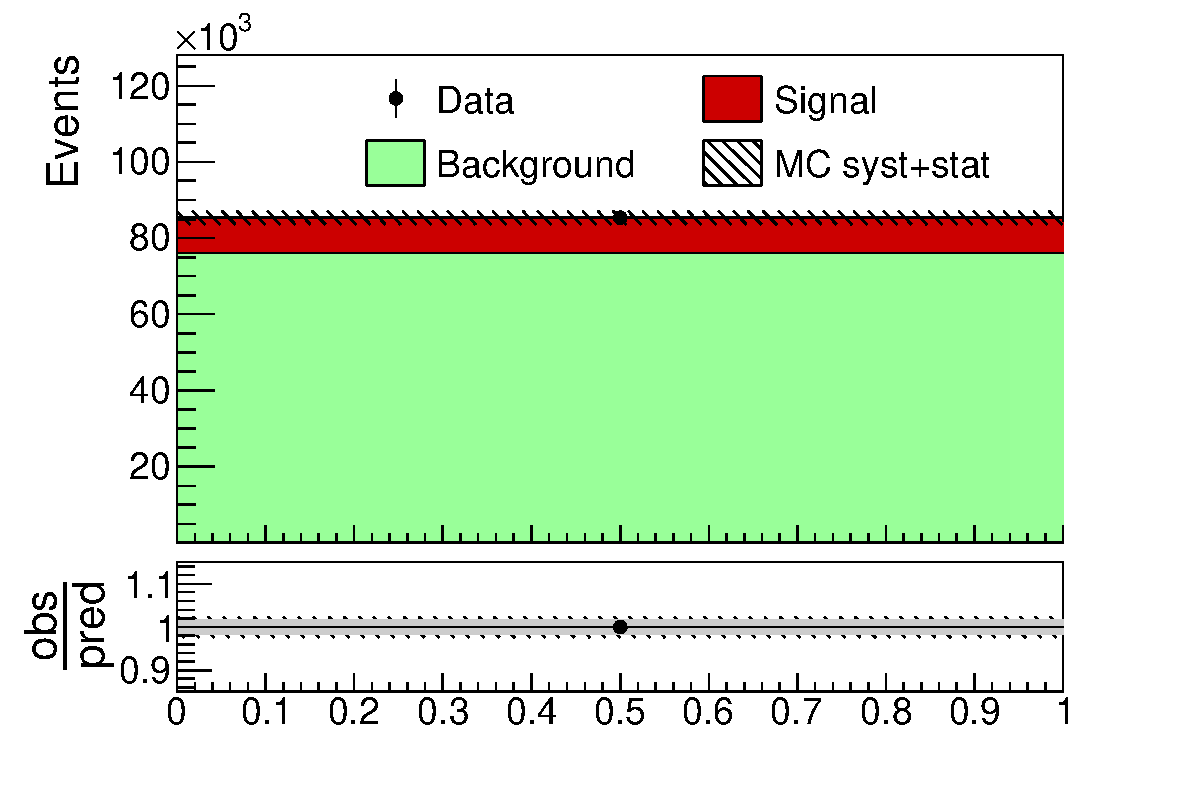
\includegraphics{Results/Figures/FitPlots/emu/total_0,0_b_jets_step_8_postfit.pdf}}
    \resizebox{0.32 \textwidth}{!}{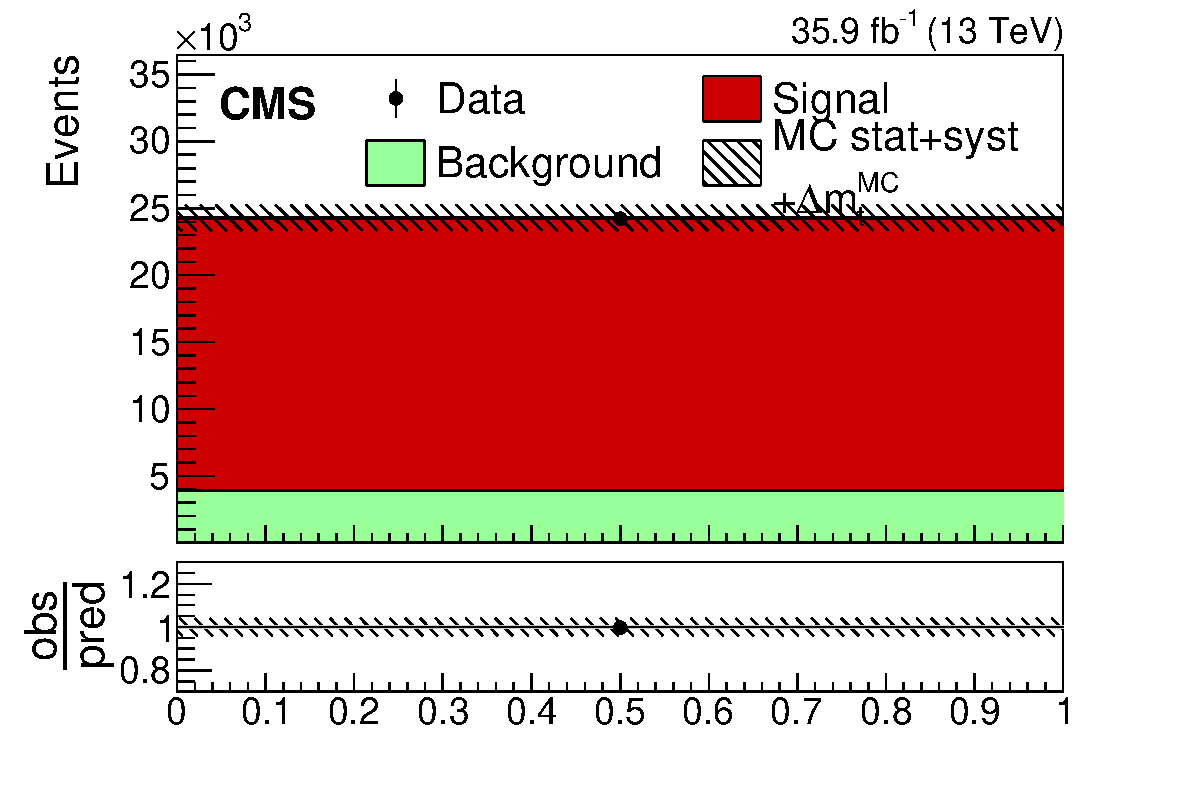
\includegraphics{Results/Figures/FitPlots/emu/total_1,0_b_jets_step_8_postfit.pdf}}
    \resizebox{0.32 \textwidth}{!}{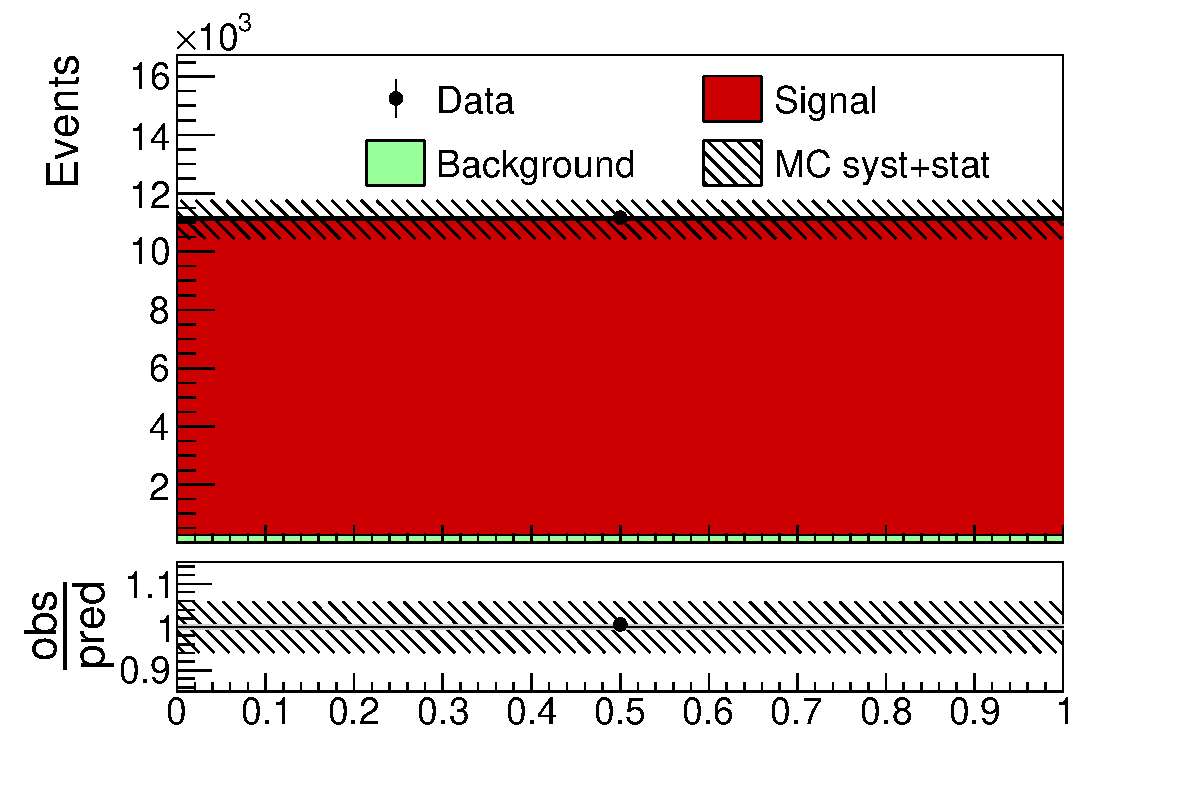
\includegraphics{Results/Figures/FitPlots/emu/total_2,0_b_jets_step_8_postfit.pdf}}

    \resizebox{0.32 \textwidth}{!}{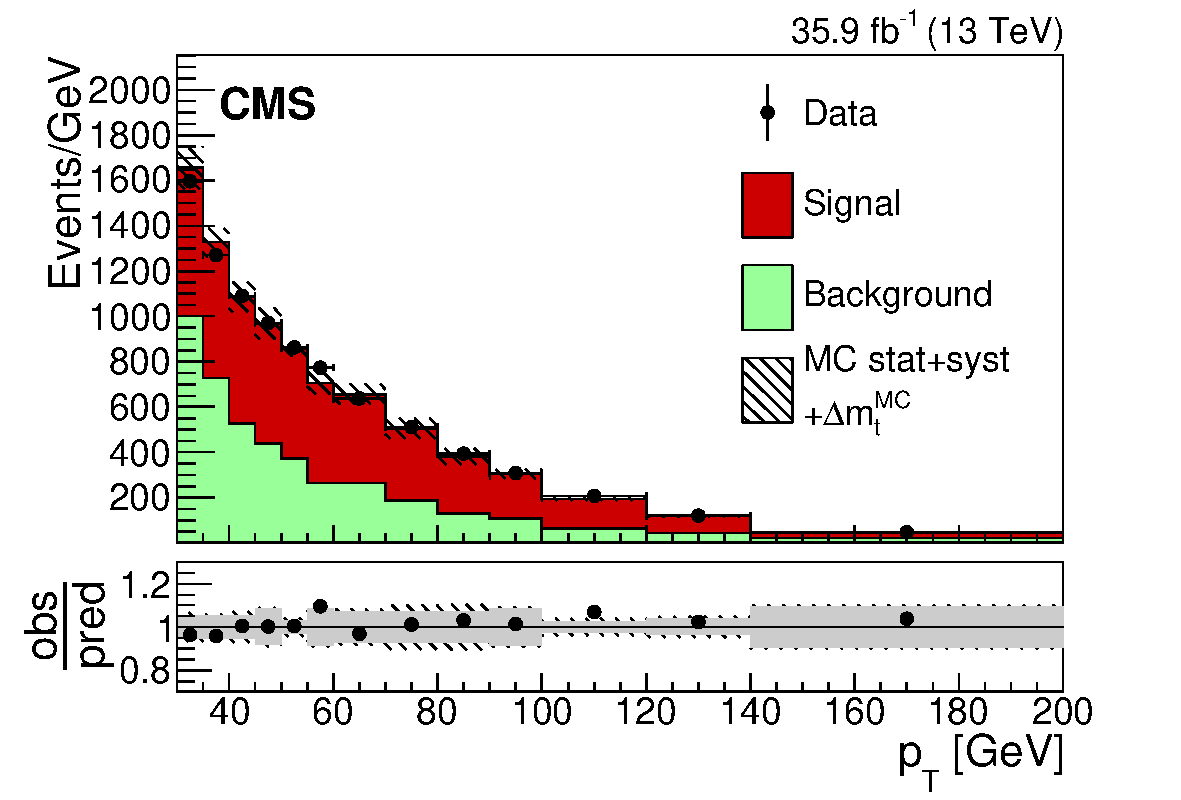
\includegraphics{Results/Figures/FitPlots/emu/lead_jet_pt_0,1_b_jets_step_8_postfit.pdf}}
    \resizebox{0.32 \textwidth}{!}{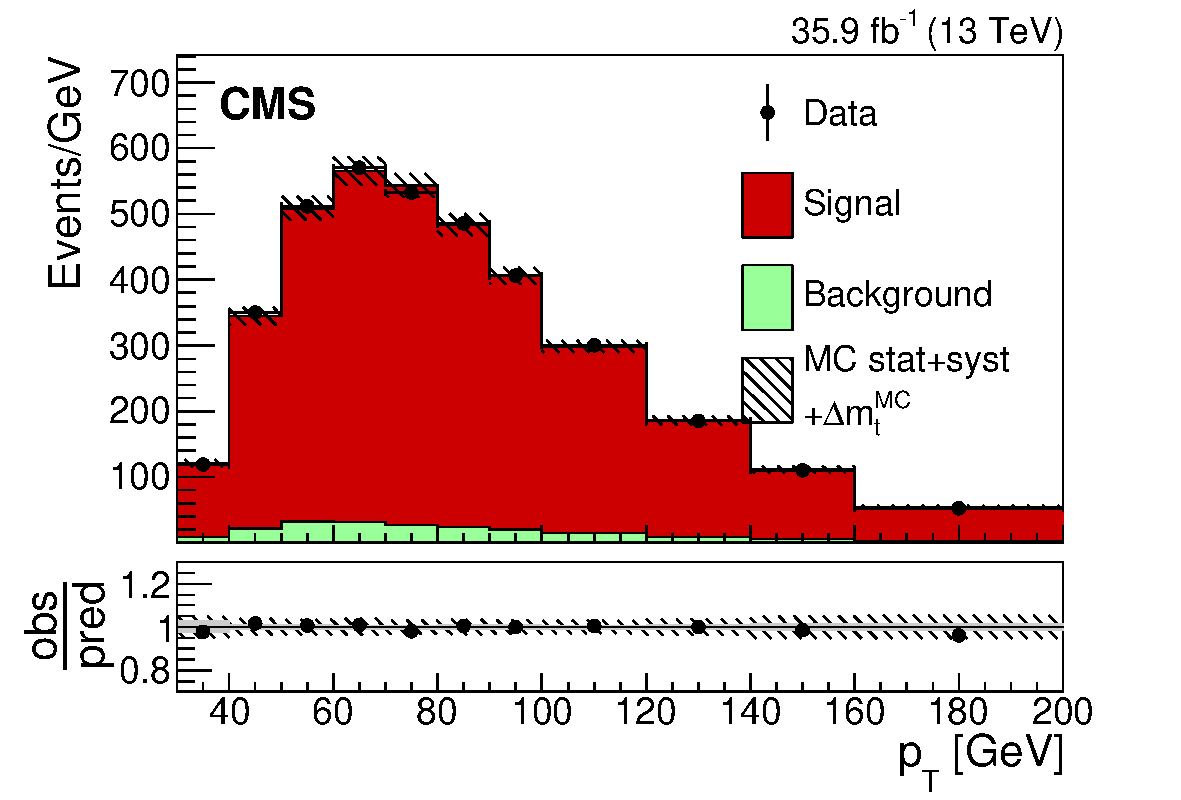
\includegraphics{Results/Figures/FitPlots/emu/lead_jet_pt_1,1_b_jets_step_8_postfit.pdf}}
    \resizebox{0.32 \textwidth}{!}{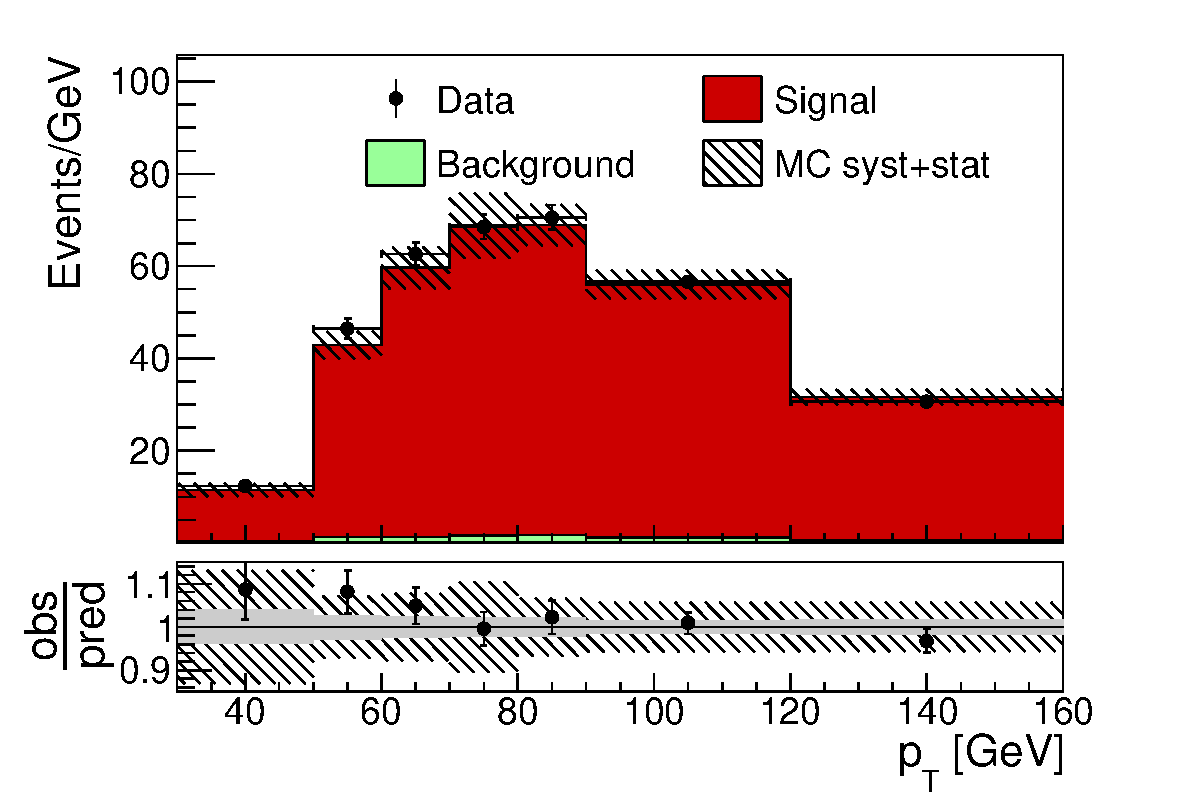
\includegraphics{Results/Figures/FitPlots/emu/lead_jet_pt_2,1_b_jets_step_8_postfit.pdf}}

    \resizebox{0.32 \textwidth}{!}{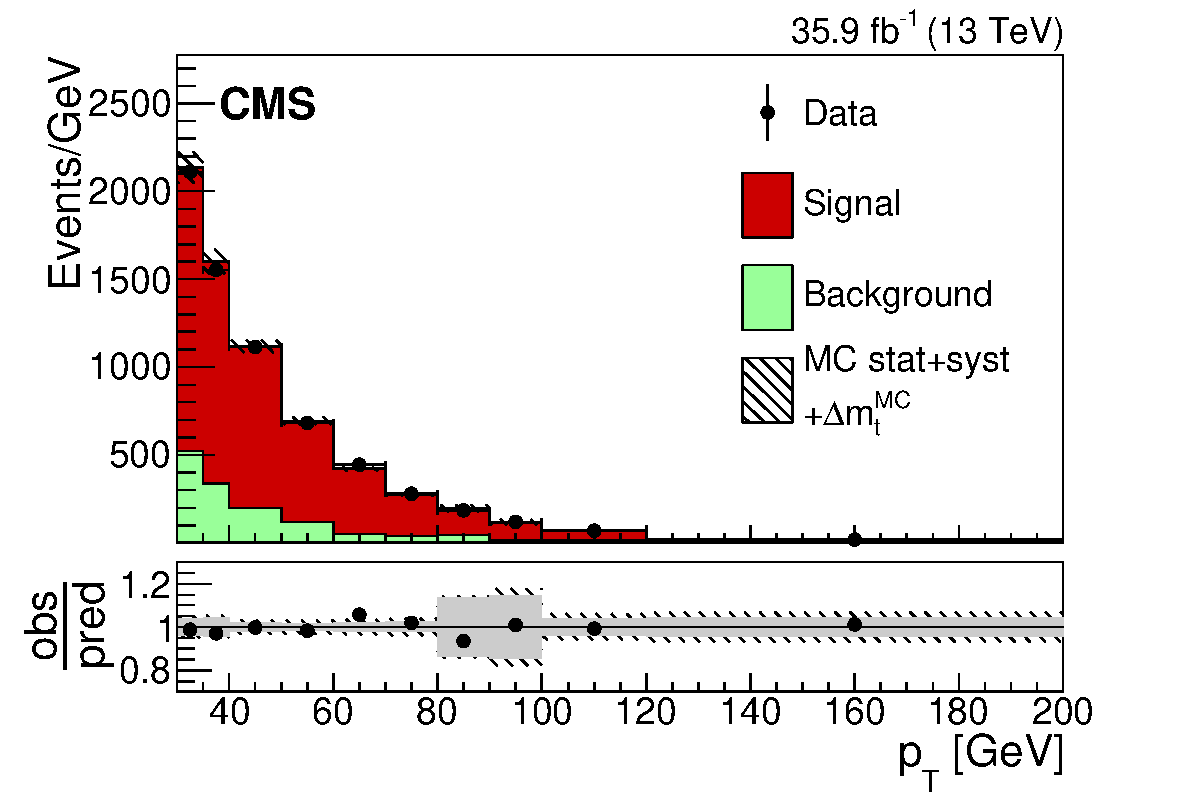
\includegraphics{Results/Figures/FitPlots/emu/second_jet_pt_0,2_b_jets_step_8_postfit.pdf}}
    \resizebox{0.32 \textwidth}{!}{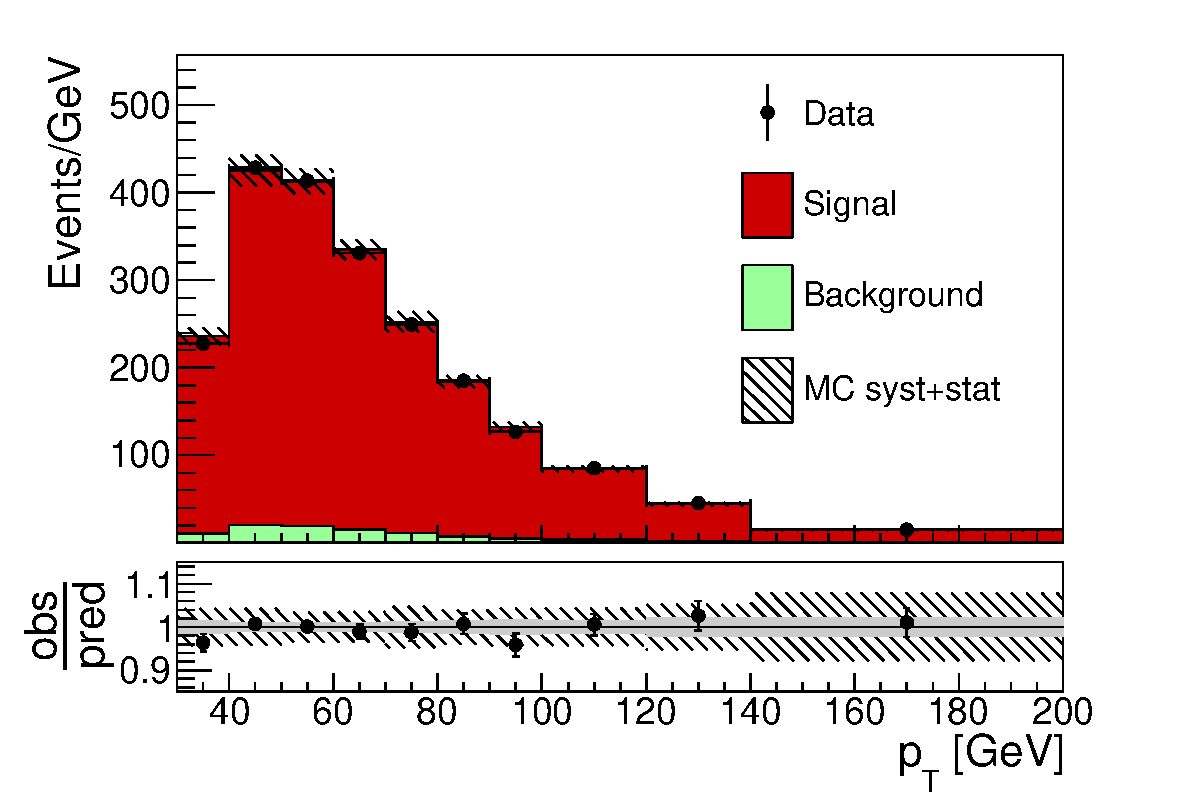
\includegraphics{Results/Figures/FitPlots/emu/second_jet_pt_1,2_b_jets_step_8_postfit.pdf}}
    \resizebox{0.32 \textwidth}{!}{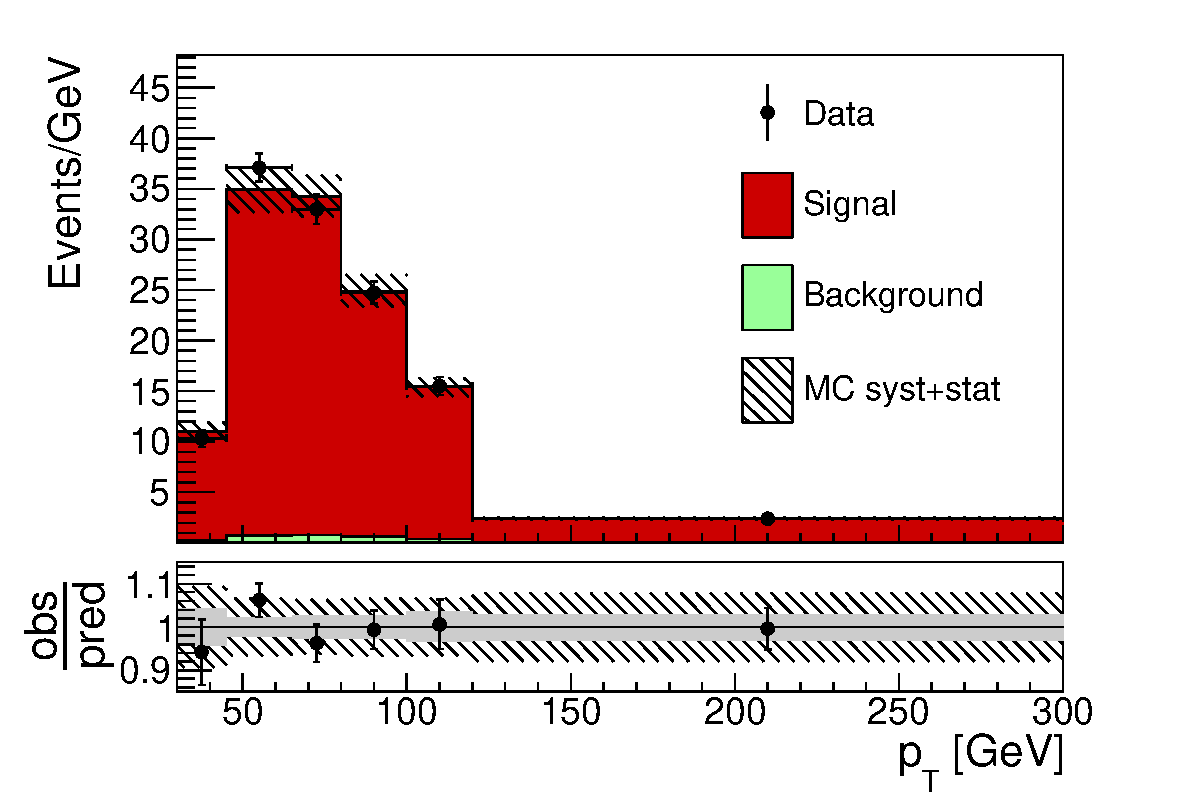
\includegraphics{Results/Figures/FitPlots/emu/second_jet_pt_2,2_b_jets_step_8_postfit.pdf}}    

    \resizebox{0.32 \textwidth}{!}{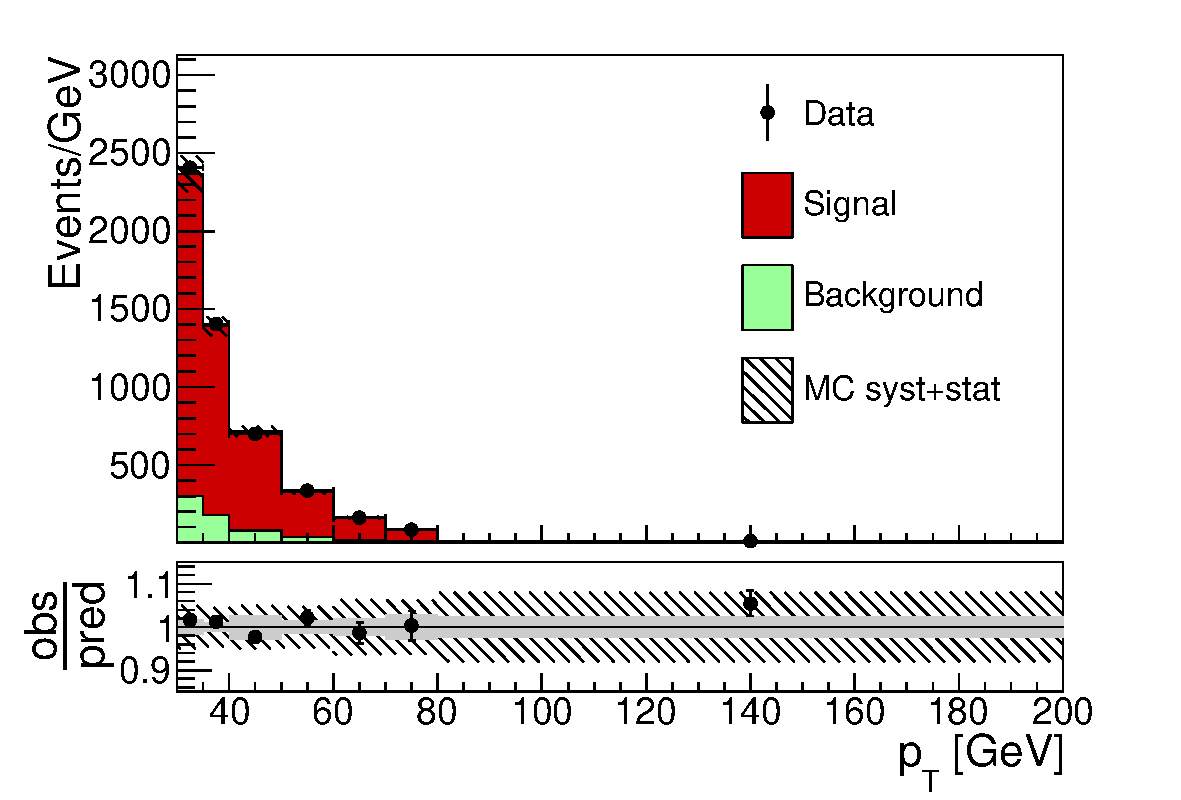
\includegraphics{Results/Figures/FitPlots/emu/third_jet_pt_0,3_b_jets_step_8_postfit.pdf}}
    \resizebox{0.32 \textwidth}{!}{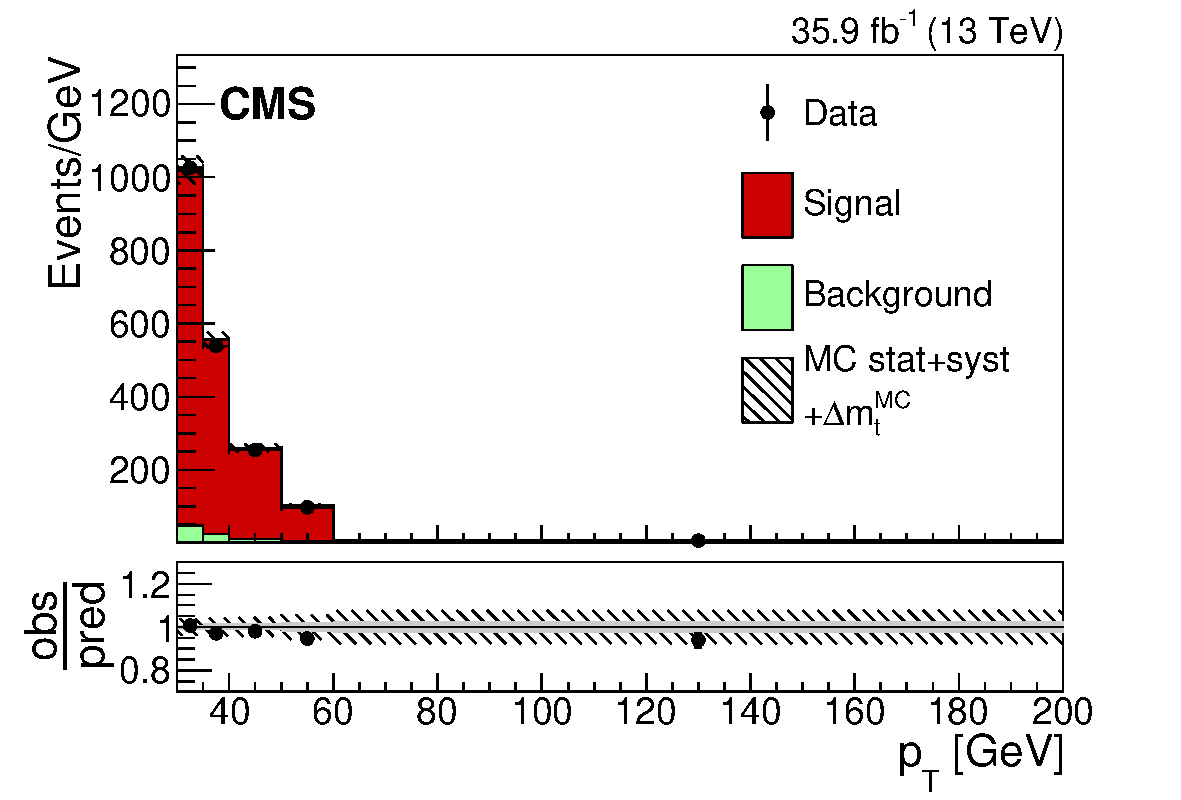
\includegraphics{Results/Figures/FitPlots/emu/third_jet_pt_1,3_b_jets_step_8_postfit.pdf}}
    \resizebox{0.32 \textwidth}{!}{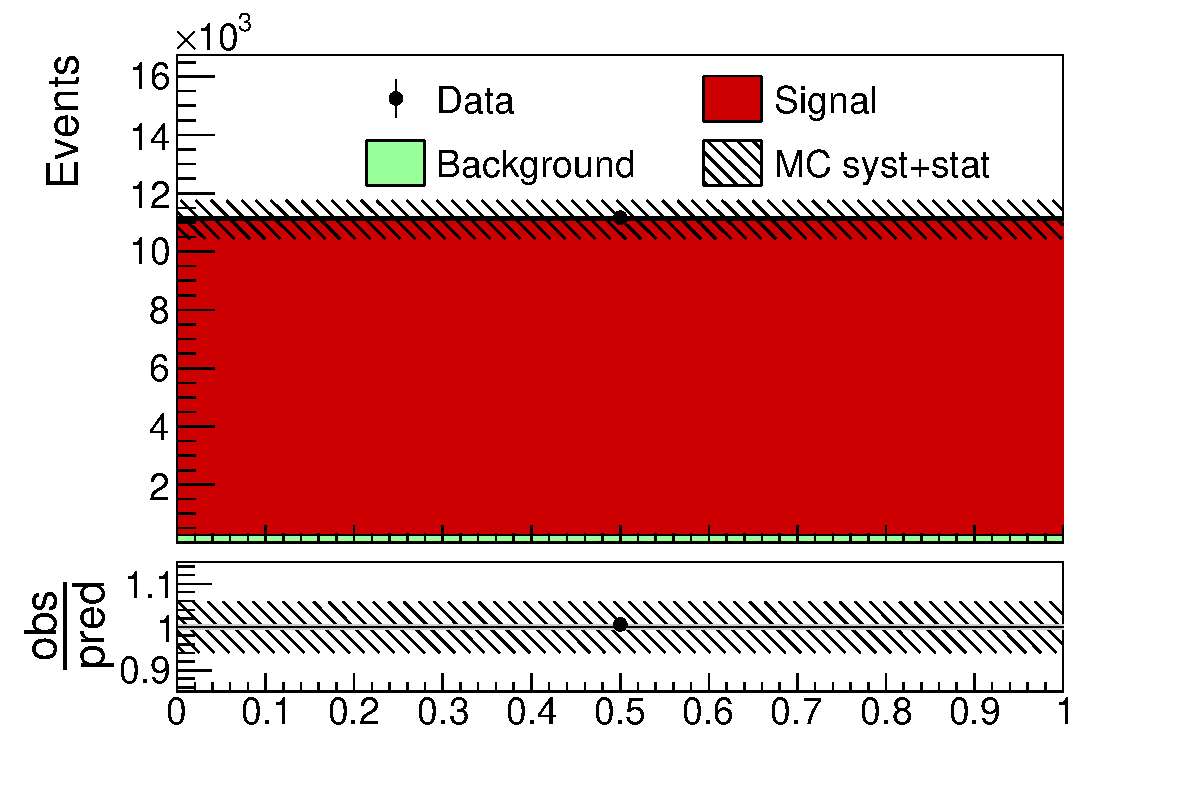
\includegraphics{Results/Figures/FitPlots/emu/total_2,3_b_jets_step_8_postfit}}   

\caption{Fitted Distributions (\emu channel) for events with zero as well as three or
  more b-tagged jets (left column): Total event yield for zero (top) and the the \pt of the jet with the lowest \pt one (second from top),
  two (second from bottom) or three or more (bottom) additional jets. The same distributions for events with one
  b-tagged jet (middle column) and two b-tagged jets (right column) are
  shown below.   
  The hatched bands correspond to the total uncertainty on the sum of
  the predicted yields. The ratios of data to the sum of the
  predicted yields are shown at the bottom of each plot. Here, the solid
  gray band represents the contribution of the statistical uncertainty.   
       \label{fig:lh_emu_postfitdistr8}}
  \end{center}
\end{figure}

\begin{figure}[htbp!]
  \begin{center}

    \resizebox{0.4 \textwidth}{!}{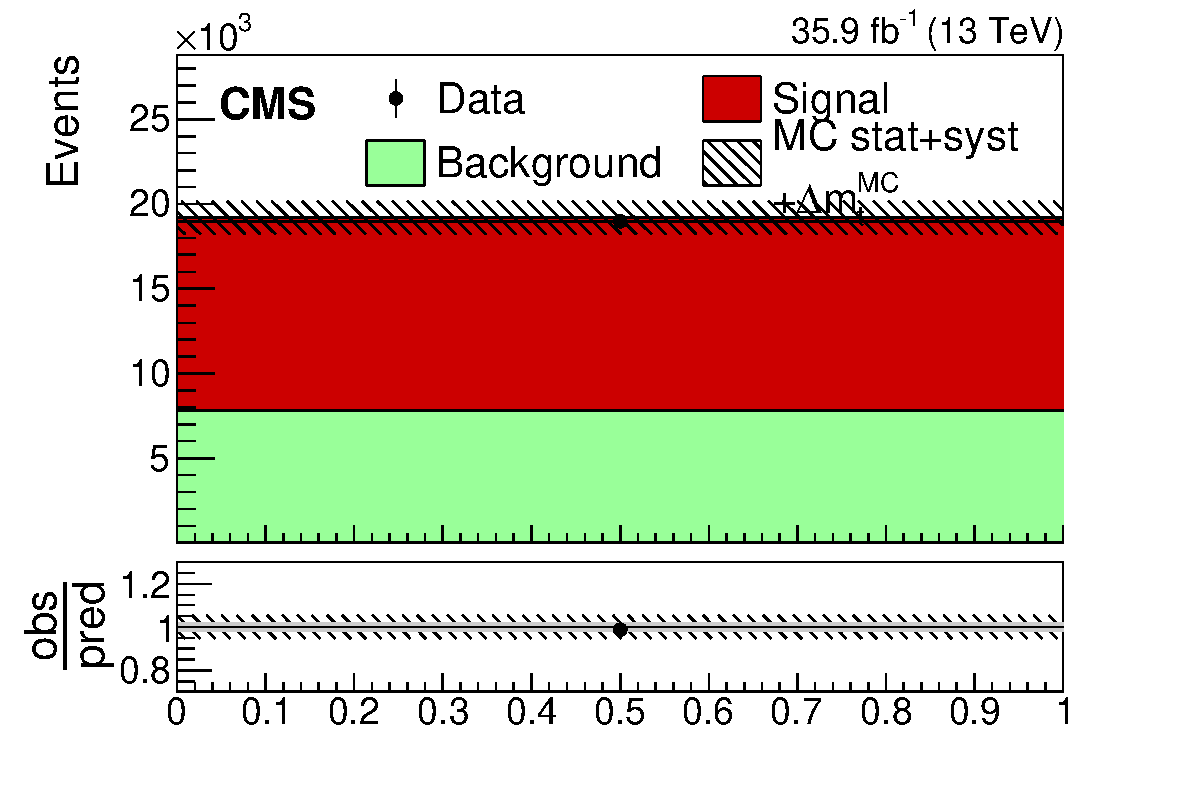
\includegraphics{Results/Figures/FitPlots/mumu/total_1,0_b_jets_step_8_postfit.pdf}}
    \resizebox{0.4 \textwidth}{!}{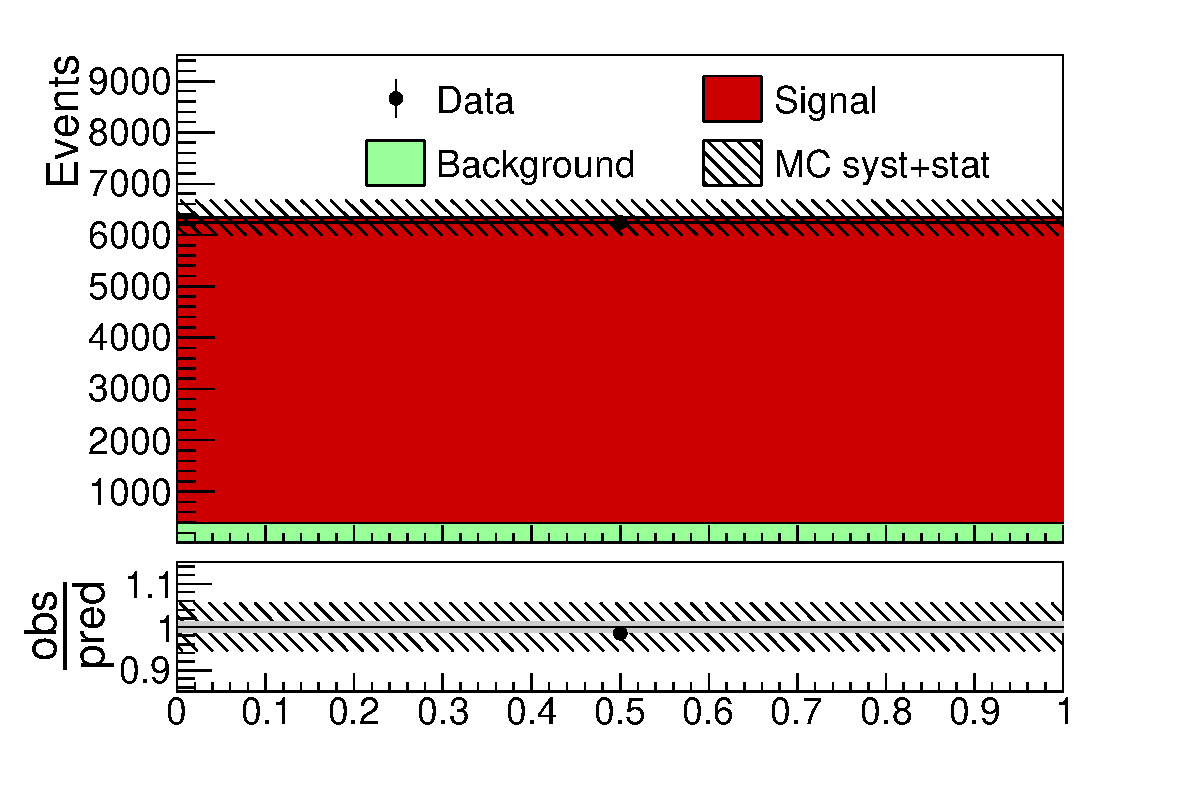
\includegraphics{Results/Figures/FitPlots/mumu/total_2,0_b_jets_step_8_postfit.pdf}}\\


    \resizebox{0.4 \textwidth}{!}{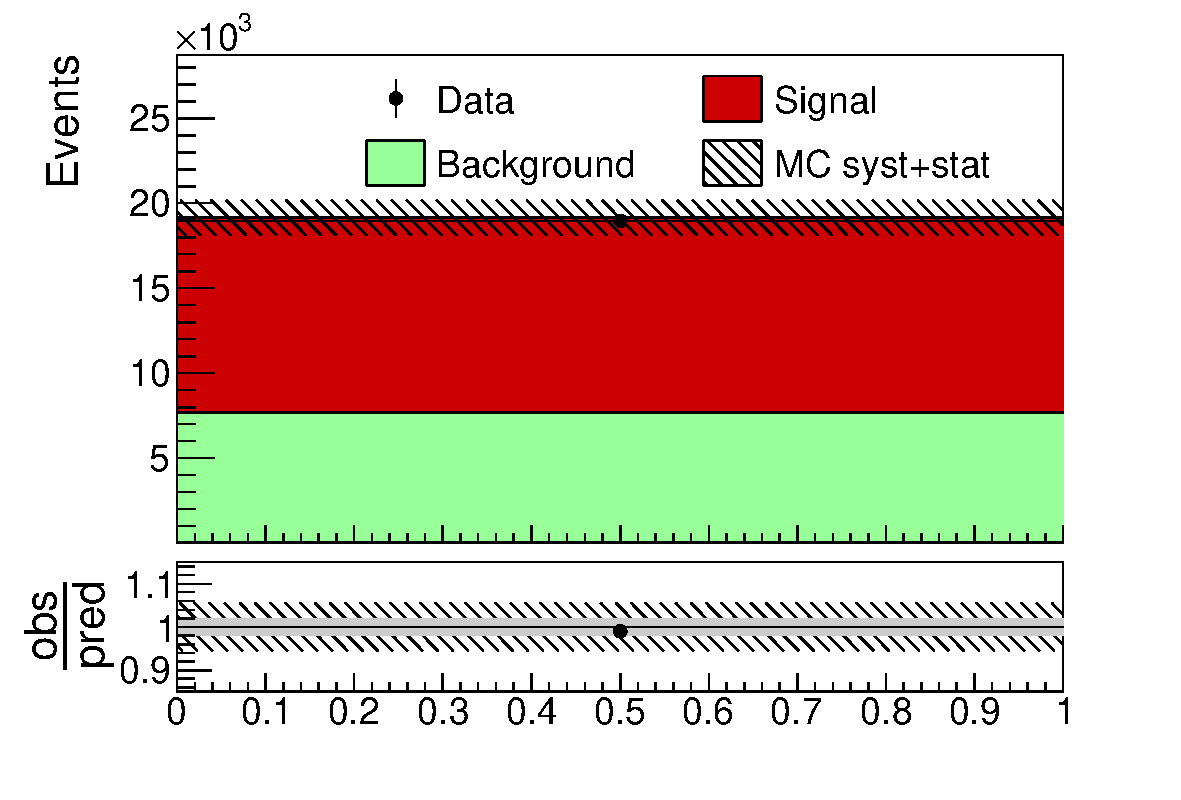
\includegraphics{Results/Figures/FitPlots/mumu/total_1,1_b_jets_step_8_postfit.pdf}}
    \resizebox{0.4 \textwidth}{!}{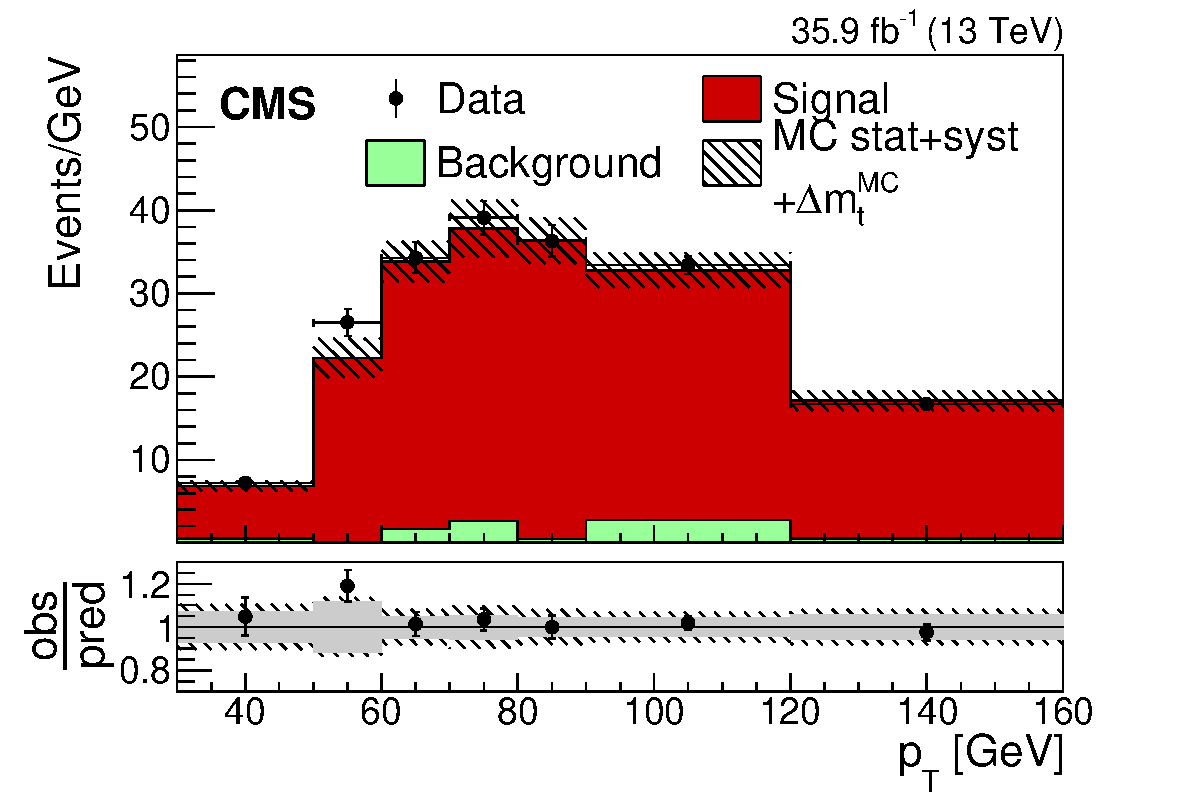
\includegraphics{Results/Figures/FitPlots/mumu/lead_jet_pt_2,1_b_jets_step_8_postfit.pdf}}\\


    \resizebox{0.4 \textwidth}{!}{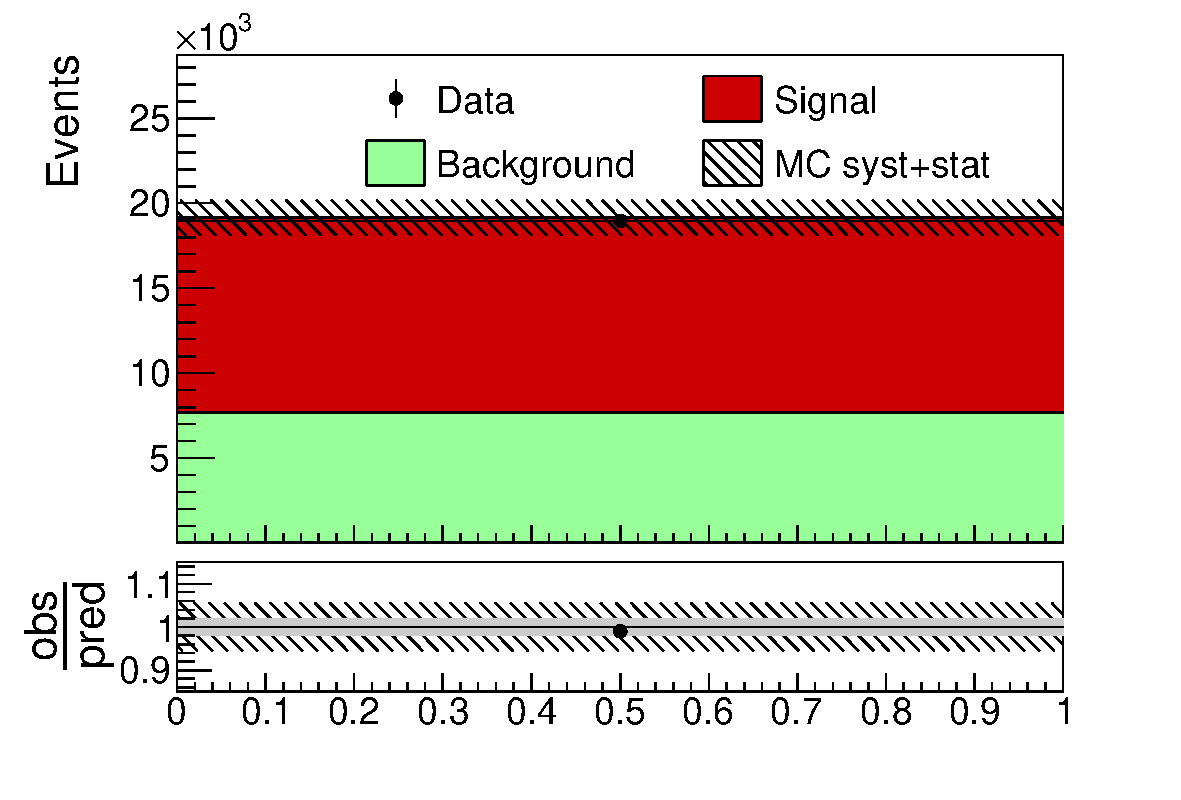
\includegraphics{Results/Figures/FitPlots/mumu/total_1,2_b_jets_step_8_postfit.pdf}}
    \resizebox{0.4 \textwidth}{!}{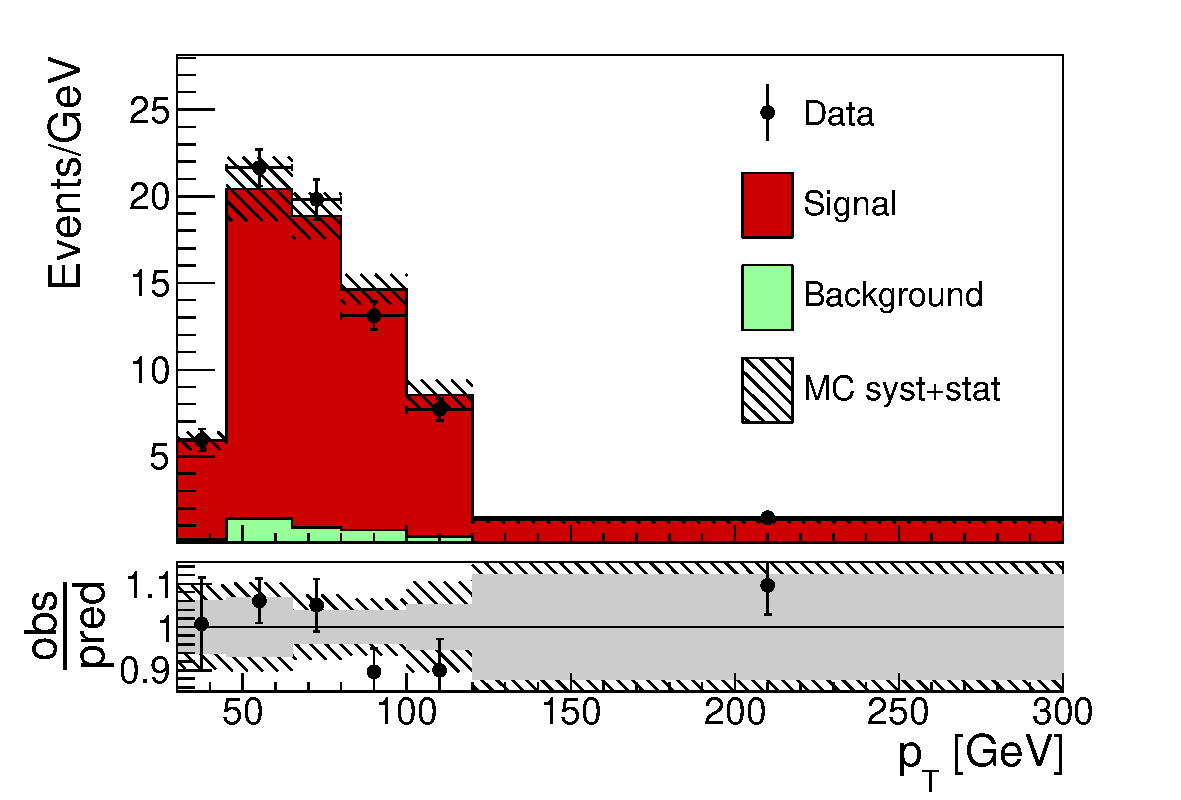
\includegraphics{Results/Figures/FitPlots/mumu/second_jet_pt_2,2_b_jets_step_8_postfit.pdf}}  \\  


    \resizebox{0.4 \textwidth}{!}{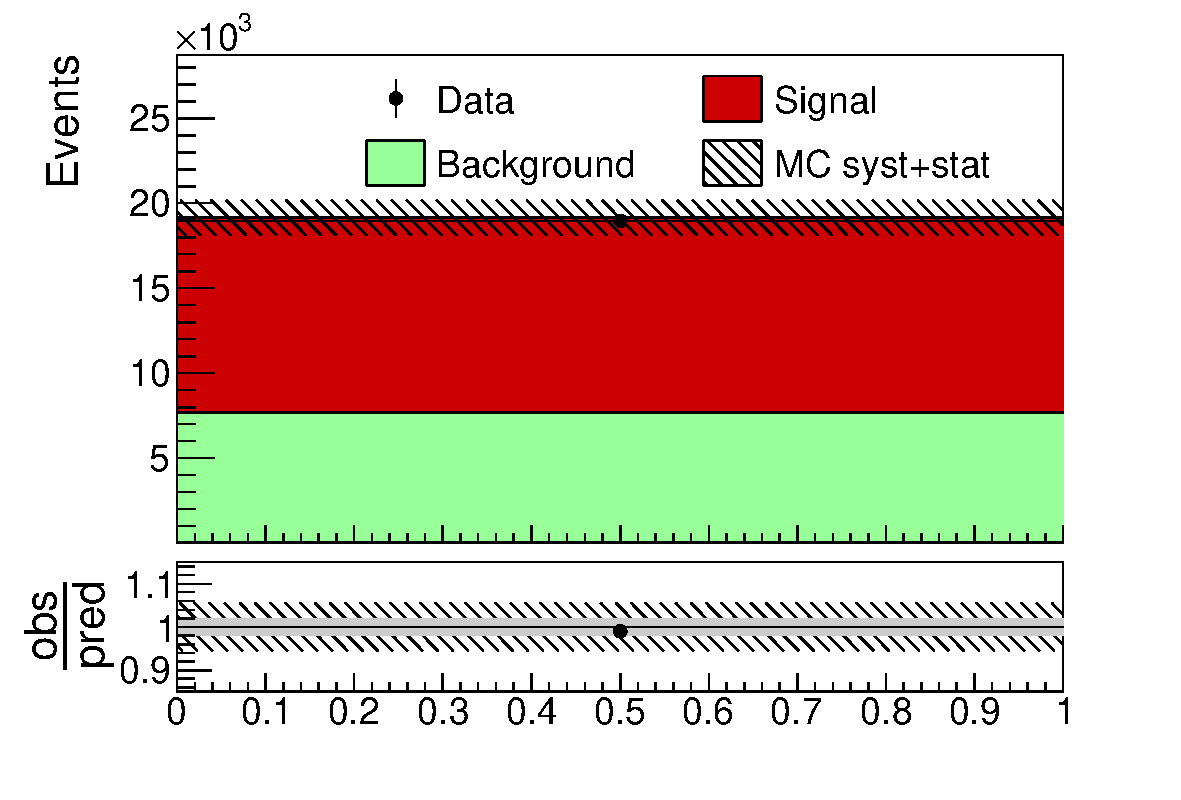
\includegraphics{Results/Figures/FitPlots/mumu/total_1,3_b_jets_step_8_postfit.pdf}}
    \resizebox{0.4 \textwidth}{!}{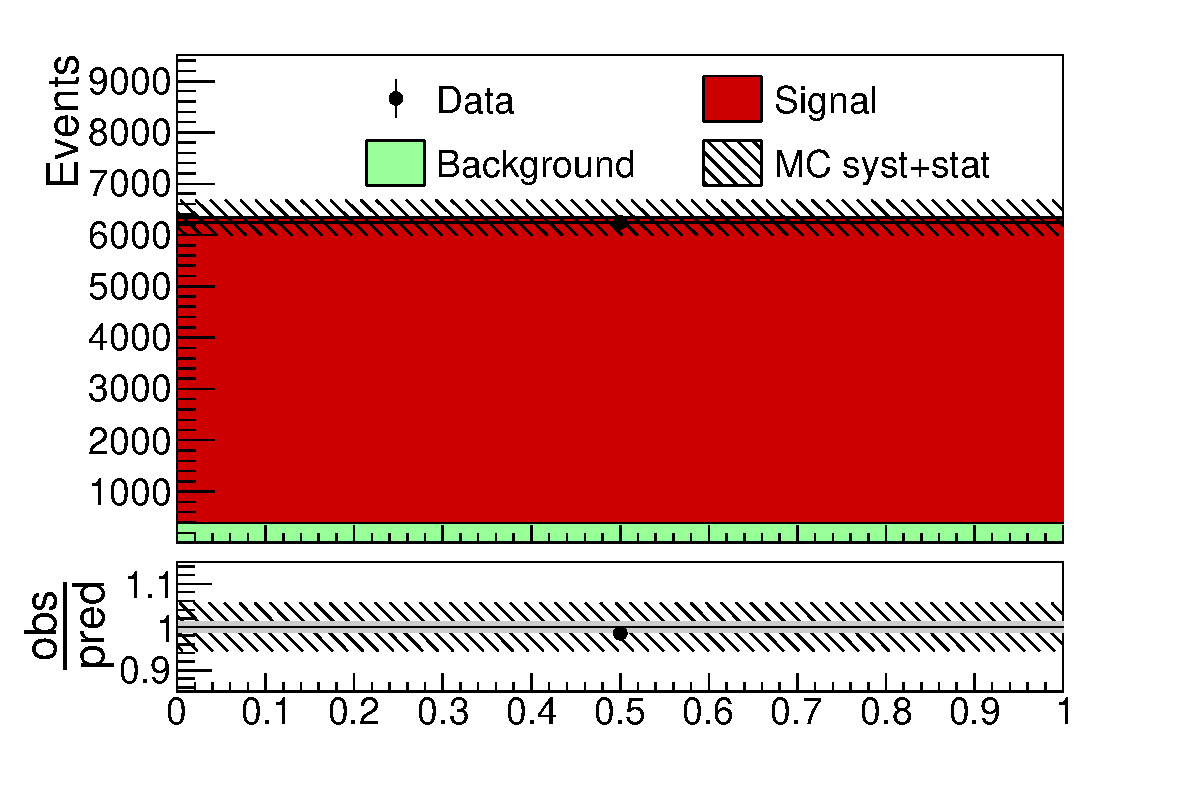
\includegraphics{Results/Figures/FitPlots/mumu/total_2,3_b_jets_step_8_postfit}}   

\caption{Fitted distributions (\mumu channel): 
  The left column shows events with one b-tagged jet and the total event yield for events with zero (top), one (second from top)
  two (second from bottom) or three or more additional jets (bottom).
  The right column shows events with two b-tagged jets and the total yield for events with zero additional jets (top),
 the \pt of the jet with the lowest \pt for one (second from top),
  two (second from bottom) or three or more (bottom) additional jets.
  The hatched bands correspond to the total uncertainty on the sum of
  the predicted yields. The ratios of data to the sum of the
  predicted yields are shown at the bottom of each plot. Here, the solid
  gray band represents the contribution of the statistical uncertainty.  
       \label{fig:lh_mumu_postfitdistr8}}
  \end{center}
\end{figure}

\begin{figure}[htbp!]
  \begin{center}
    \resizebox{0.4 \textwidth}{!}{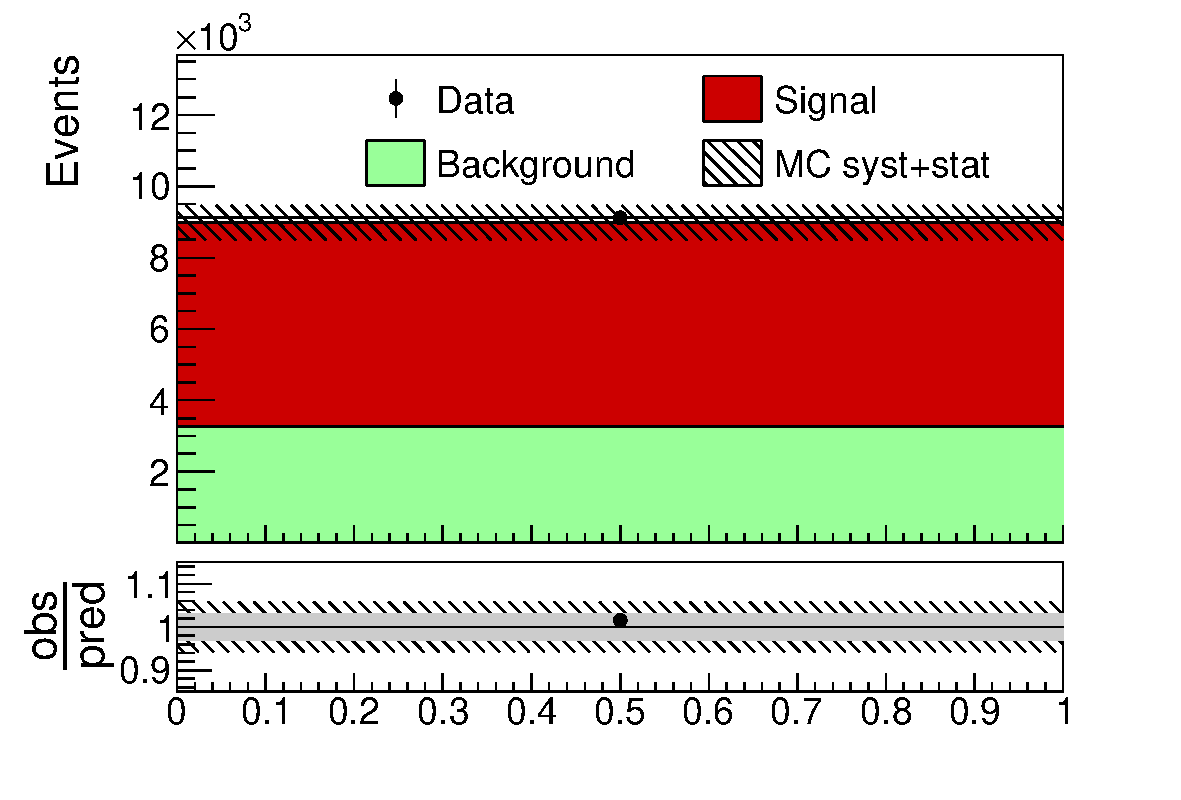
\includegraphics{Results/Figures/FitPlots/ee/total_1,0_b_jets_step_8_postfit.pdf}}
    \resizebox{0.4 \textwidth}{!}{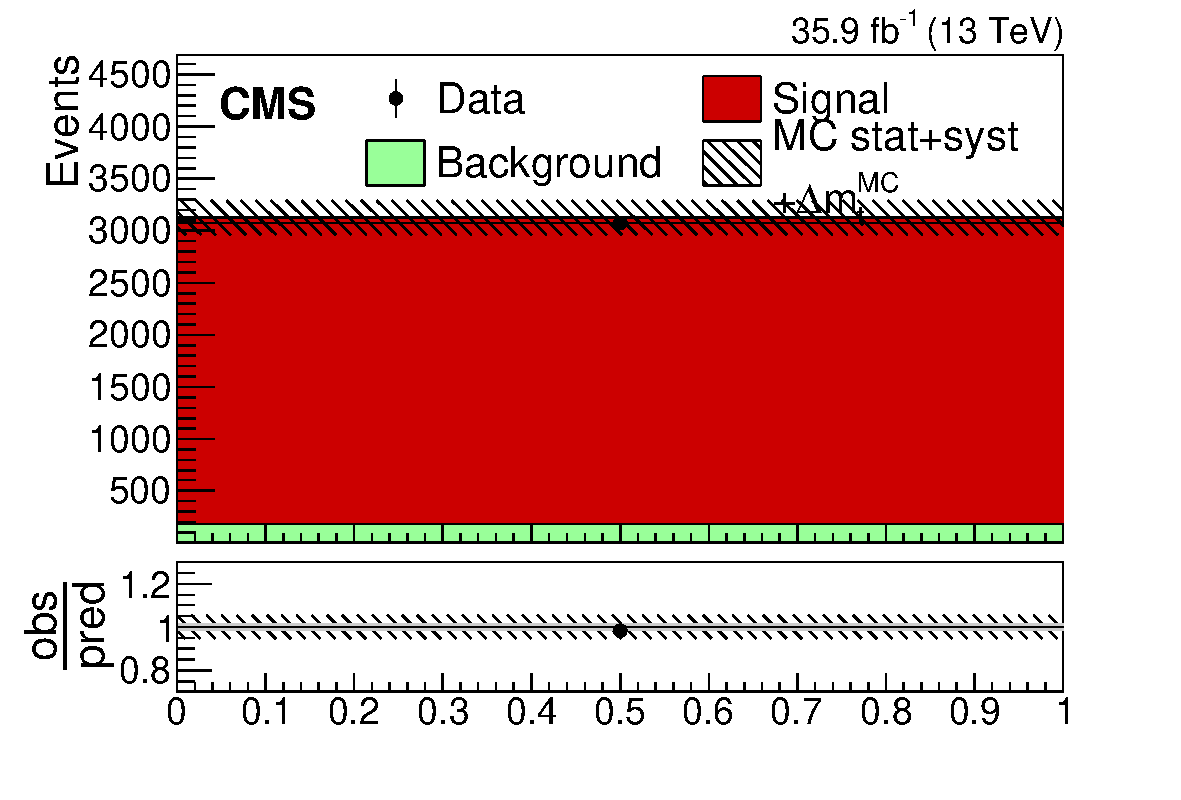
\includegraphics{Results/Figures/FitPlots/ee/total_2,0_b_jets_step_8_postfit.pdf}}\\

    \resizebox{0.4 \textwidth}{!}{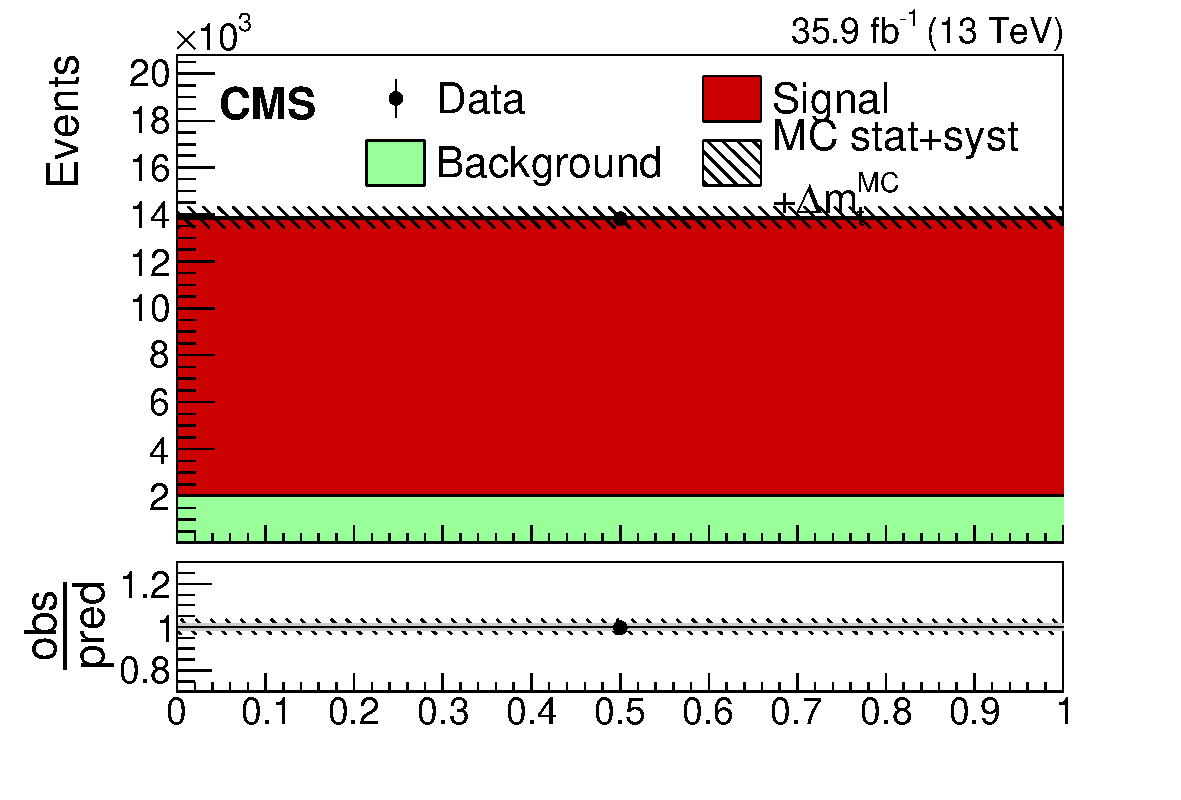
\includegraphics{Results/Figures/FitPlots/ee/total_1,1_b_jets_step_8_postfit.pdf}}
    \resizebox{0.4 \textwidth}{!}{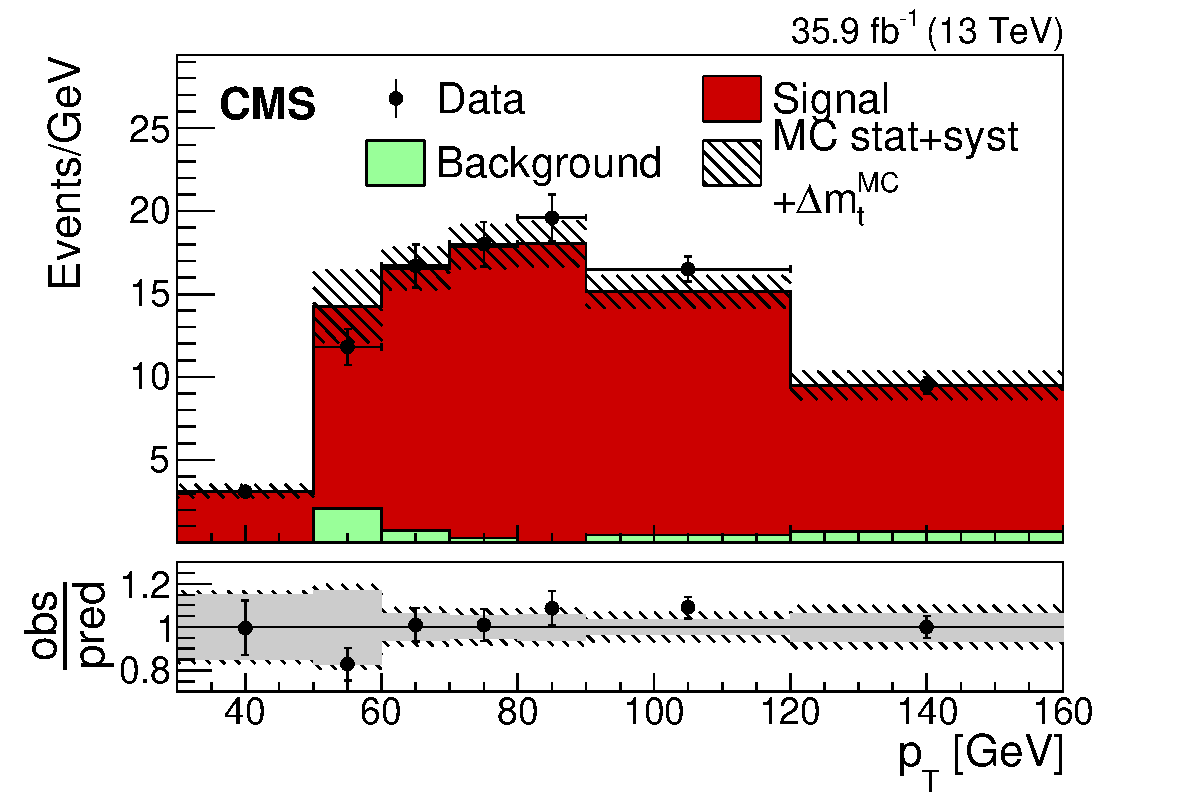
\includegraphics{Results/Figures/FitPlots/ee/lead_jet_pt_2,1_b_jets_step_8_postfit.pdf}}\\

    \resizebox{0.4 \textwidth}{!}{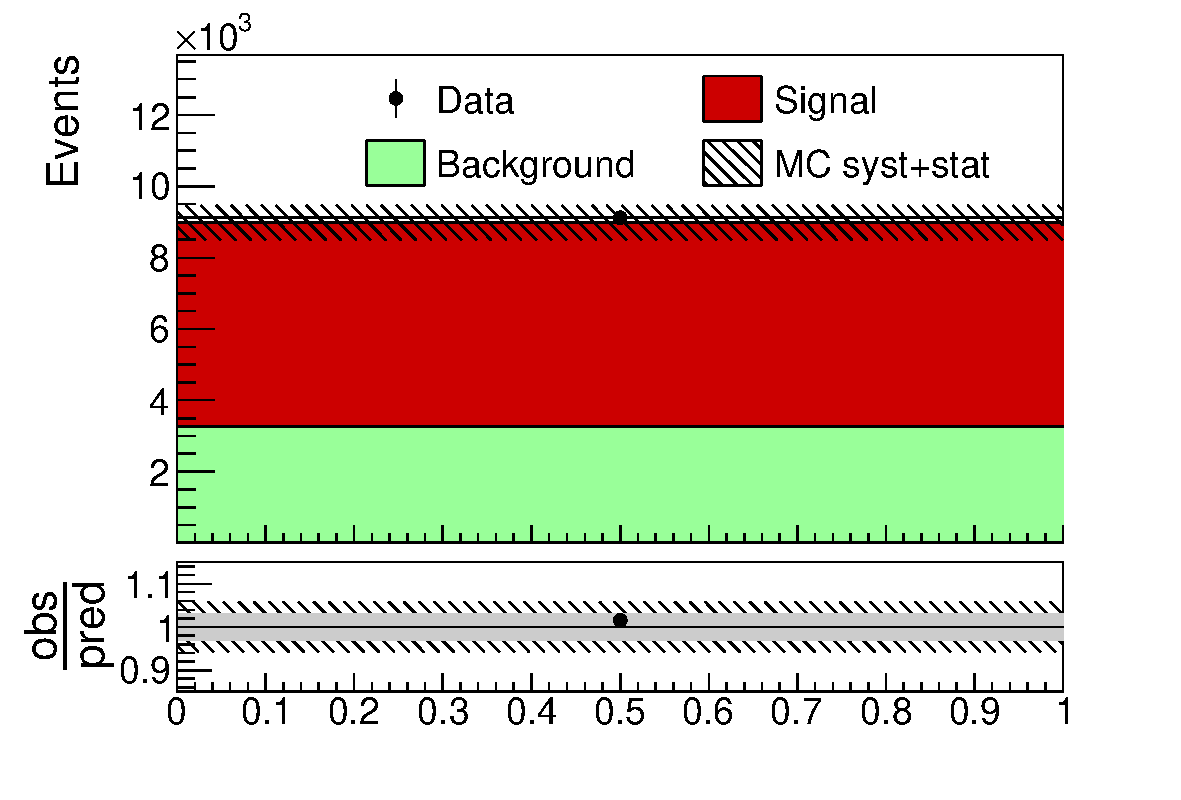
\includegraphics{Results/Figures/FitPlots/ee/total_1,2_b_jets_step_8_postfit.pdf}}
    \resizebox{0.4 \textwidth}{!}{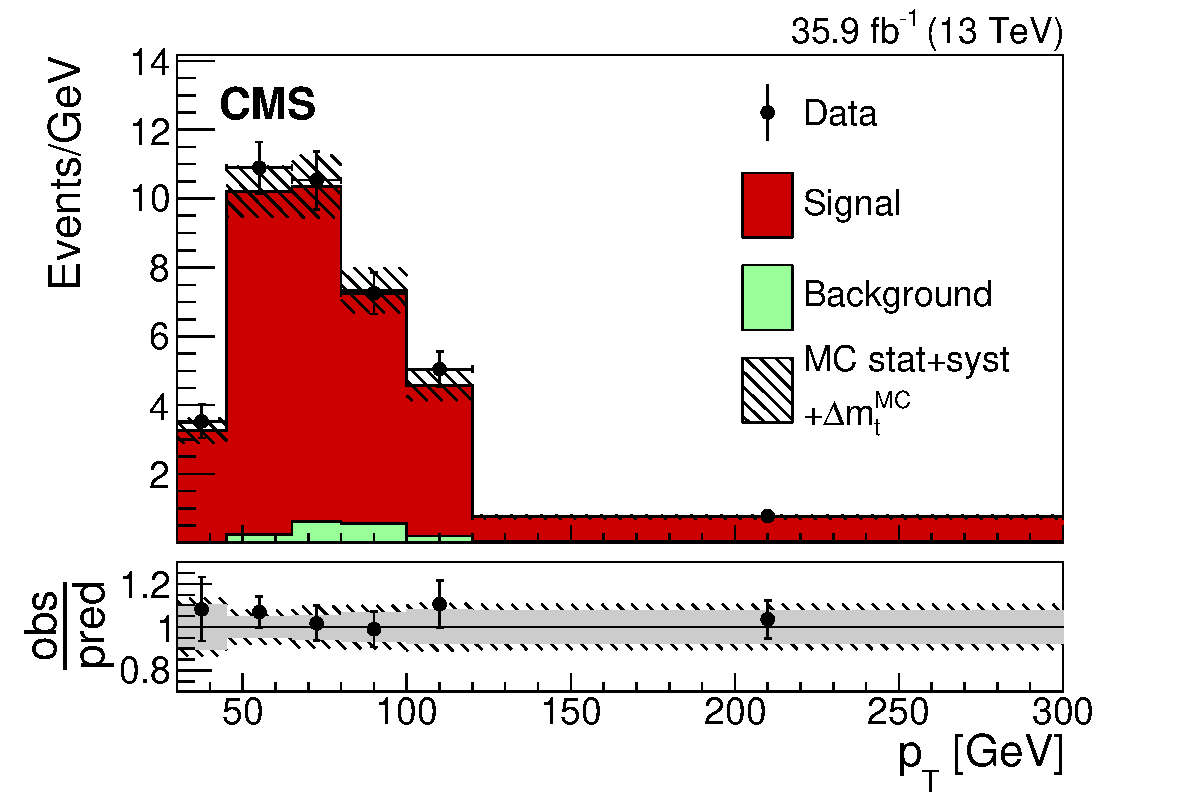
\includegraphics{Results/Figures/FitPlots/ee/second_jet_pt_2,2_b_jets_step_8_postfit.pdf}} \\   

    \resizebox{0.4 \textwidth}{!}{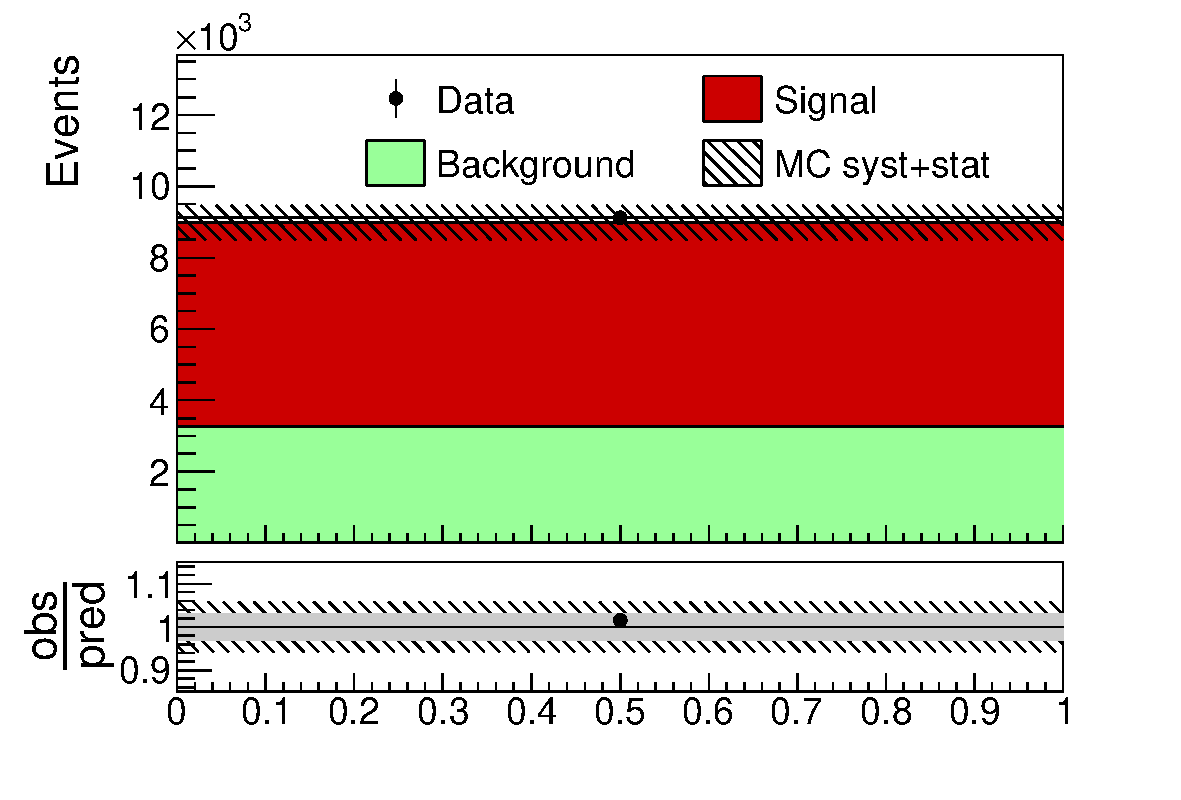
\includegraphics{Results/Figures/FitPlots/ee/total_1,3_b_jets_step_8_postfit.pdf}}
    \resizebox{0.4 \textwidth}{!}{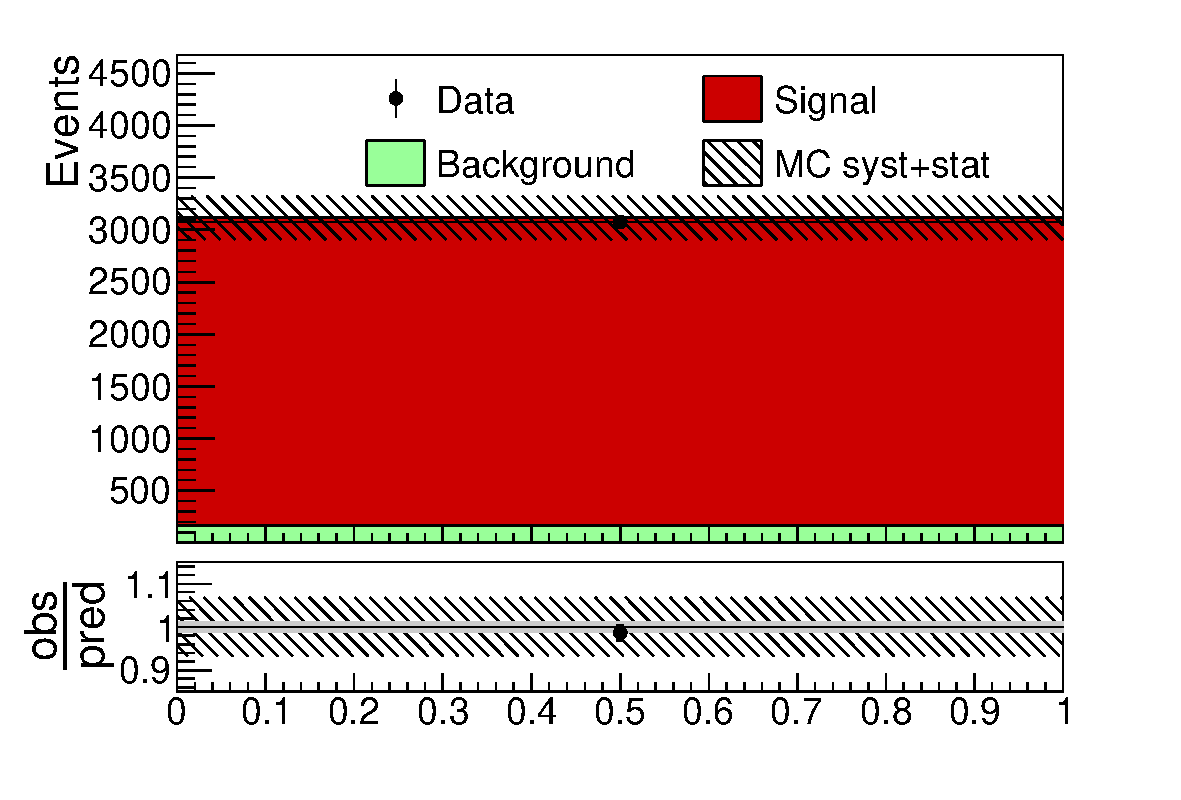
\includegraphics{Results/Figures/FitPlots/ee/total_2,3_b_jets_step_8_postfit}}   

\caption{Fitted distributions (\ee channel): 
  The left column shows events with one b-tagged jet and the total event yield for events with zero (top), one (second from top)
  two (second from bottom) or three or more additional jets (bottom).
  The right column shows events with two b-tagged jets and the total yield for events with zero additional jets (top),
 the \pt of the jet with the lowest \pt for one (second from top),
  two (second from bottom) or three or more (bottom) additional jets.
  The hatched bands correspond to the total uncertainty on the sum of
  the predicted yields. The ratios of data to the sum of the
  predicted yields are shown at the bottom of each plot. Here, the solid
  gray band represents the contribution of the statistical uncertainty.  
       \label{fig:lh_ee_postfitdistr8}}
  \end{center}
\end{figure}

The plots show that simulation agrees with the data after applying the fitted parameters.
The agreement can be expected and shows that the fit succesfully scales simulation to data and the
 simulation is able to model the data within its uncertainties.
The post-fit uncertainties are smaller compared to the plots showing the non-constrained uncertainties in Figure \ref{fig:xsec_emu_inputdistr},\ref{fig:xsec_mumu_inputdistr} and \ref{fig:xsec_ee_inputdistr}, which
shows their constraints from the fit.


\subsection{Results for systematic uncertainties}
\label{sec:results_uncert}

As described in Section \ref{sec:xsec_stat} the results of the fit include the \ttbar cross section value as well as the results for the fitted nuisance parameters.
For the nuisance parameters a fitted value (also called pull) of $0$ stands for the nominal result, while a value of $\pm 1$ stands for the $\pm 1 \; \sigma$ variation.
The impact of each of the nuisance parameters on the cross section is estimated by fixing one nuisance parameter to the nominal value and repeating the fit.
The reduction in the resulting uncertainty on the cross section is then considered as the contribution of that single uncertainty. This calculation does not consider correlations between multiple uncertainties,
so the quadratic sum of the contributions of all uncertainties does not correspond to the total uncertainty.

Table \ref{tab:lh_res_eightsimple} shows the contributions from the most relevant uncertainties. Suitable uncertainty sources are combined.
It also shows the result for the cross section itself and for the extrapolation of the full to the visible phase space including the extrapolation of the relevant uncertainties.
Figure \ref{fig:res_pulls} shows the pulls and constraints for the most relevant systematic uncertainties.
The contributions of all single uncertainty sources, together with their pulls and constraints are shown in Appendix \ref{app:uncert}.


\begin{table}[htbp!]
\center
\caption{Results of the \ttbar cross section at $\sqrt{s}= 13 \TeV$ with the full 2016 dataset. The systematic uncertainties are broken down by their sources. The uncertainty from the luminosity is externalised from the fit
and not included in the table. 
\label{tab:lh_res_eightsimple}}
\begin{tabular}{ l |  c }
 \hline
Name & Contribution [\%] \\ \hline
Trigger & ${0.3}$ \\
Lepton ID/isolation & ${2.1}$ \\
Lepton energy scale/resolution & ${0.1}$ \\
Jet energy scale & ${0.4}$ \\
Jet energy resolution & ${ < 0.1}$ \\
B-tag & ${0.2}$ \\
Mistag & ${0.1}$ \\
Pile-up & ${0.2}$ \\
$t\bar{t}$ ME scale & ${0.2}$ \\
tW ME scale & ${< 0.1}$ \\
PDF & ${1.1}$ \\
Top $p_{T}$ & ${0.5}$ \\
ME/PS matching & ${0.1}$ \\
UE tune & ${0.3}$ \\
$t\bar{t}$ FSR scale & ${0.5}$ \\
$t\bar{t}$ ISR scale & ${0.2}$ \\
tW FSR scale & ${< 0.1}$ \\
tW ISR scale & ${< 0.1}$ \\
B-hadron BR & ${0.1}$ \\
fragmentation & ${0.4}$ \\
CR QCD-inspired & ${0.3}$ \\
tW background & ${1.1}$ \\
DY background & ${1.0}$ \\
Diboson background & ${0.3}$ \\
$t\bar{t}$ background & ${0.3}$ \\
W+jets background & ${0.2}$ \\
Stat & ${0.2}$ \\
Total vis & ${2.6}$ \\ \hline
$\sigma_{t\bar{t}}$(13 TeV) vis & 24.88 pb \\ \hline
$t\bar{t}$ ME scale (extr) & $\mp^{0.3}_{0.1}$ \\
PDF (extr) & $\pm^{0.8}_{0.6}$ \\
Top $p_{T}$ (extr) & $\mp^{0.8}_{0.0}$ \\
$t\bar{t}$ ISR scale (extr) & $\mp^{0.1}_{0.0}$ \\
$t\bar{t}$ FSR scale (extr) & $\pm^{0.1}_{0.0}$ \\
UE tune (extr) & $\mp^{0.0}_{0.0}$ \\
 \hline
Total & $\pm^{2.9}_{2.6}$ \\ \hline
$\sigma_{t\bar{t}}$(13 TeV) & 827 pb \\ \hline \hline
\end{tabular}
\end{table}

\begin{figure}[htbp!]
  \begin{center}

    \resizebox{0.45 \textwidth}{!}{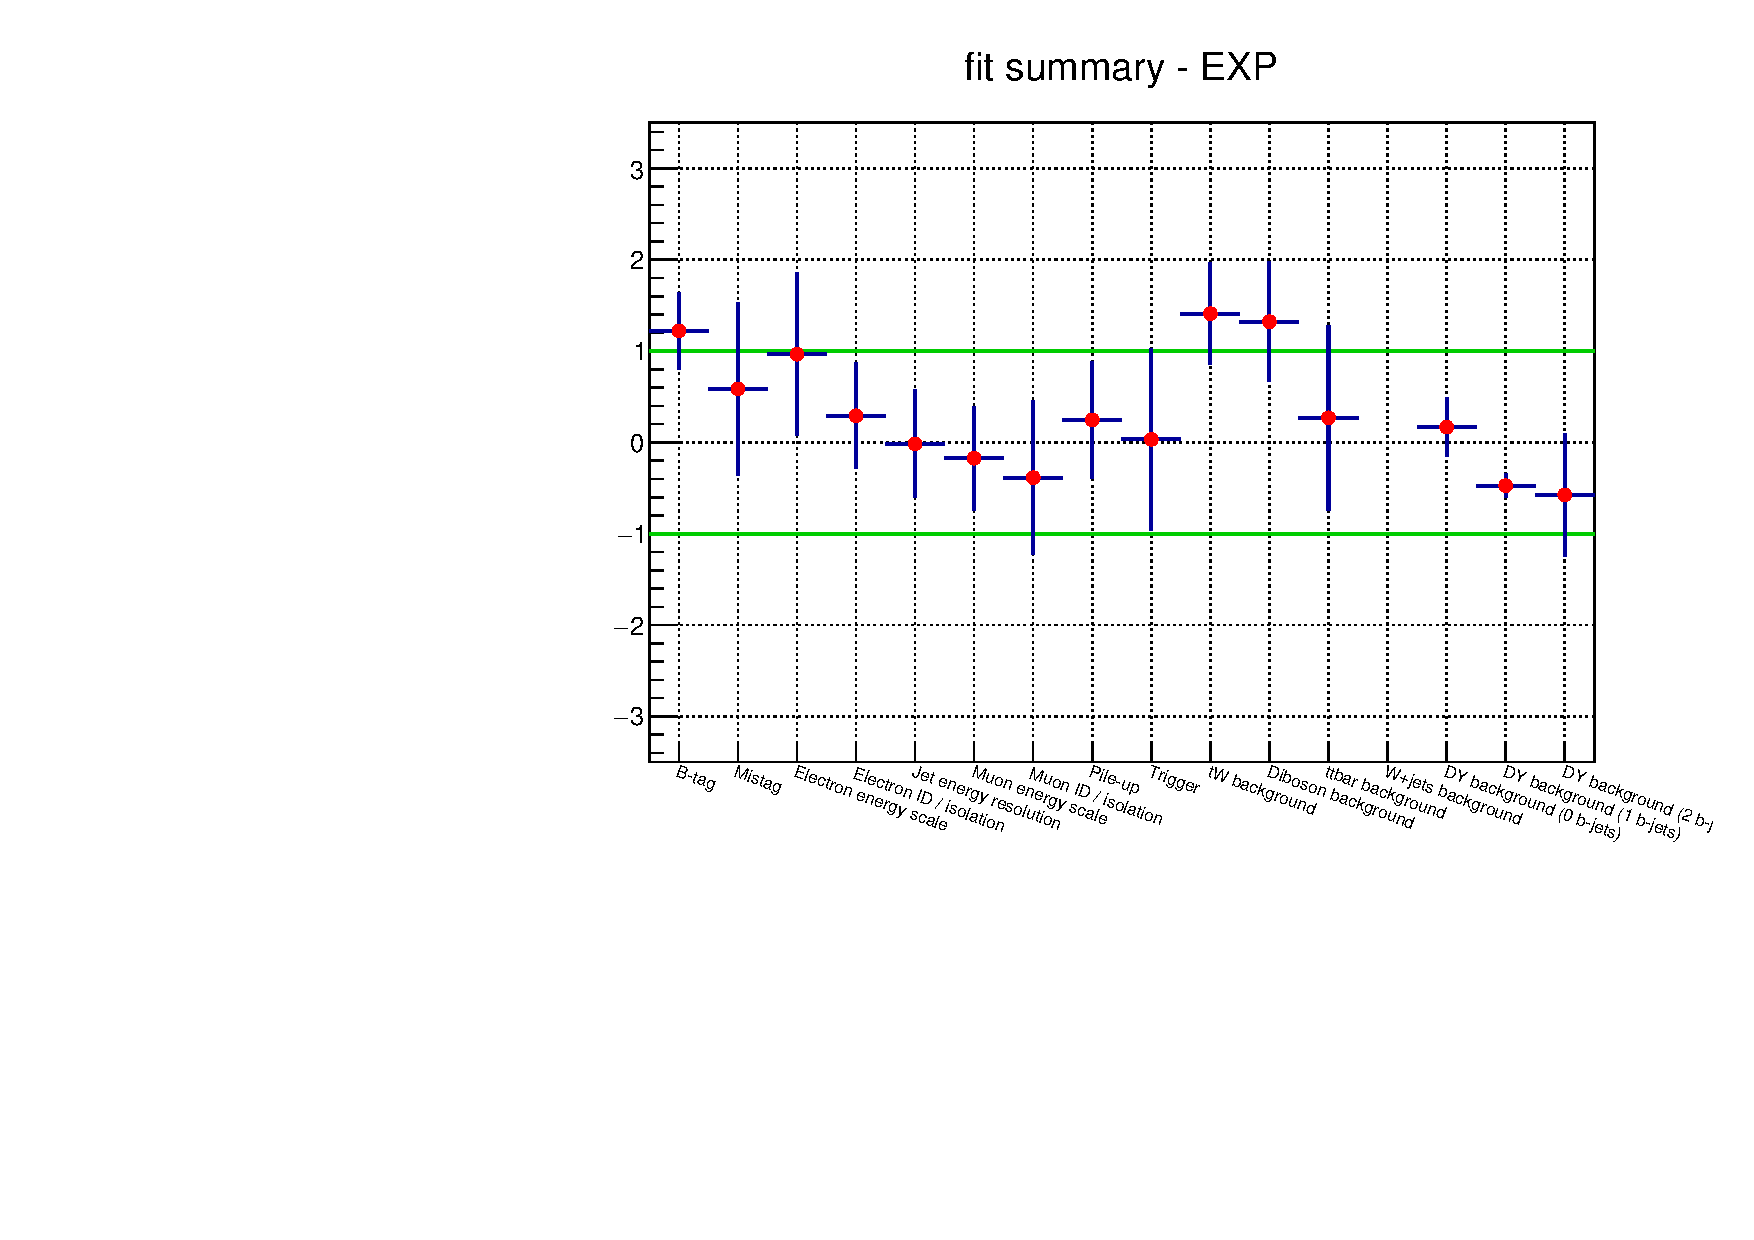
\includegraphics{Results/Figures/FitPlots/all_fitSummary.pdf}}
    \resizebox{0.45 \textwidth}{!}{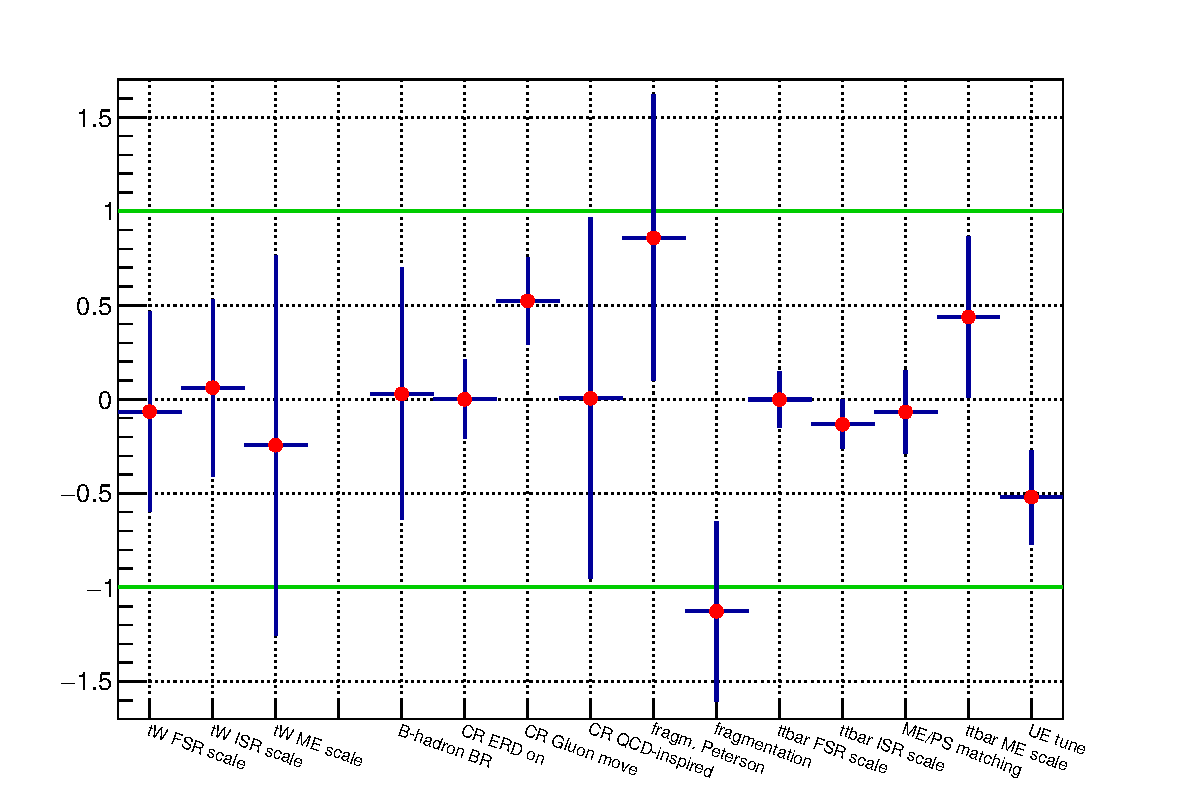
\includegraphics{Results/Figures/FitPlots/mod_fitSummary.pdf}}   

\caption{Pulls and constraints of relevant experimental (left) and theoretical (right) systematic uncertainties. 
       \label{fig:res_pulls}}
  \end{center}
\end{figure}

The results for the lepton (electron and muon) ID uncertainties can be described together as they are highly correlated.
As described in Section \ref{sec:xsec_templates}, the higher of the two uncertainties (the electron uncertainty) is constrained and
the lower of the two (the muon uncertainty) is largely unconstrained. Compared to the constraints, the values for the pulls 
are small. The lepton uncertainties have the largest contribution to the total uncertainty from all single uncertainties with about $\sim 2 \%$. 

% The overall impact of the electron energy resolution uncertainty is small, its pull is close to zero and it is hardly constrained showing
% that the analysis is not sensitive to the effect.
% The electron energy scale uncertainty has a pull to $\sim -1.2$ with a constraint of $\sim 0.6 \; \sigma$, the impact on the total uncertainty however is comparatively small.

% The muon energy scale uncertainty (also including resolution effects) does not have any large impact on the analysis, nor is it pulled or constrained.

Since the trigger uncertainty is an overall normalization uncertainty on all templates, its size directly propagates to the final uncertainty, but it is neither pulled nor constrained.  

% Most of the jet energy scale uncertainty sources have only little impact on the final uncertainty. 

% The jet energy resolution uncertainty has little impact on the uncertainty on the measured cross section. The pull of $\sim 1.1$ is not showing any real tension with the prediction considering the constraint of $0.81 \; \sigma$.

% The uncertainty related to the b-tagging efficiency can be constrained to about $0.5 \; \sigma$ since the efficiency itself is determined intrinsically as explained in Section \ref{sec:xsec_stat}.
% The effect on the total uncertainty is comparatively large despite the constraint with about $0.5 \; \%$.
% The nuisance paremeter is fitted to a value of $0.6$ which does not deviate significantly from the nominal value considering the constraint.
% The uncertainty on the rate to b-tag a jet not originating from a b-quark (mistag rate) only has a small impact on the uncertainty of the cross section and it is not significantly constrained.

% The uncertainty related to the pile-up contributes about $0.3 \; \%$ to the total uncertainty on the measured cross section. It is hardly constrained  ($0.82 \; \sigma$) and the pull at $0.5$ is consistent with the nominal value.
% This result shows that the cross section measurement is not sensitive to the deviation of the pile up description in simulation shown in Figure \ref{fig:control_var_PU}.

% The uncertainty related to the B-hadron decay branching ratio only does not significantly contribute to the uncertainty on the measured cross section. It is slightly constrained to about $0.7 \; \sigma$ and the fitted value of the nuisance parameter is below $0.1$.

% The uncertainties related to the B-Hadron fragmentation contribute to the order of $0.7 \; \%$ and $0.3 \; \%$ to the uncertainty of the measured cross section for the model internal uncertainty and for the Peterson model uncertainty respectively.
% Both uncertainties are constrained to the range of $0.4 - 0.6 \; \%$ and the pulls are consistent with the nominal value. 
% Again the constraint shows the sensitivity of the analysis to uncertainties related to b-quarks.

 The 28 uncertainty sources for the PDF are related to the uncertainty for the PDF represented in eigenvectors.
 They contribute to the uncertainty on the measured cross section up to about $0.4\%$ per individual uncertainty. Overall, they are not strongly constrained and the pull hardly differs from the nominal value.
 During the extrapolation of the cross section from the visual to the full phase space the PDF uncertainties contribute again, as described in Section \ref{sec:xsec_extraction}, in the order of $1.1  \%$ in total.

 Other theoretical uncertainties do not significantly contribute to the total uncertainty, since they are either constrained or their impact is small.

% The impact of the uncertainty from the reweighting of the \pt of the top quark on the final measured cross section is negligible.
% The fitted results corresponds to the systematic variation. This variation is obtained by correcting the simulation according to a measurement of the differtial top \pt distribution and can consequently
% be expected to describe the measured data better than the nominal variation.


% As shown in Figures \ref{fig:control_var_TT_ISRSCALE} and \ref{fig:control_var_TT_FSRSCALE} the ISR and FSR scale uncertainties affect the template distributions used for the fit.
% The large variations lead to a strong constraint of about $0.2 \; \sigma$ and a contribution to the final uncertainty of $0.6 \;\%$ and $0.3 \; \%$ to for the FSR and ISR scale respectively.
% A uniform distribution is assumed for the behaviour of the nuisance parameter, but the pull is still consistent with the nominal value.
% Both the ISR and FSR scale uncertainties only make small additional contributions to the uncertainty on the extrapolation of the cross section.

% The impact of the uncertainty of the matching of matrix element generator and parton shower on the uncertainty of the measured cross section is comparatively small with $0.15 \%$. 
% It is heavily constrained to $0.2 \; \sigma$ and the fitted value for the nuisance parameter is consistent with the nominal value.
% The uncertainty on the underlying event behaves similarly: It impacts the final uncertainty on the order of $0.2 \; \%$ is constrained to $0.26 \; \sigma$ and consistent with the nominal value.

% The highest impact from the three uncertainties related to the model of color reconnection contributes $0.14 \; \$$ to the uncertainty on the measured cross section, while the contribution from the other two models is negligible.
% The variation is strongly constrained to about $0.1 \; \sigma$ and the pull is consistent with zero.

% Background events containing a W and jets or a \ttbar pair not decaying into two leptons do not significantly contribute to the overall number of events.
% The uncertainty from the variation of the respective cross sections is negligible. The variations are hardly constrained and the pulls are consistent with zero.

% Events containing two bosons mostly contain no b-tagged jet, so they do not significantly contribute to the distributions most sensitive to the \ttbar contribution. This results in a contribution of the uncertainty on the di-boson production cross section on the measured \ttbar cross section of $0.2 \; \%$
% The variation of the di-boson production cross section is hardly constrained and the fitted result is consistent with the nominal cross section.
Events containg a single top quark and a W boson behave very similar to events from \ttbar production. The cross section of tW production is low compared to the cross section of \ttbar production, but due to the similarities between
both types of events there is still a considerable impact. The uncertainty on the tW production cross section has an impact of about $1.1 \%$ on the measured \ttbar cross section.

The uncertainty on the production cross section of Drell-Yan events is explicitely decorrelated according to the number of b-tagged jets (corresponding to the event categorisation in the fit).
Added in quadrature the total contribution to the total uncertainty is $1\%$.


\section{Comparison to theory predictions and previous results}
\label{sec:results_comp}

The cross section in the full phase space is found to be:
\begin{equation}
\stt  =  \resultxsecmain.
\end{equation}
 
This result is in agreement with the theoretical prediction for the \ttbar production cross section calculated with the \textsc{Top++} program~\cite{Czakon:2011xx} at NNLO in perturbative QCD, including soft-gluon resummation to the next-to-next-to-leading log~\cite{Andreev:2017vxu} of :
\begin{equation}
\stt = \xsectheo.
\end{equation}

This measurement is also in agreement with a previous CMS measurements of the \ttbar production cross section in the dilepton channel \cite{Khachatryan:2016kzg}:
\begin{equation}
\sttbar = 815 \pm  9 ({\rm stat}) \pm 38 ({\rm syst}) \pm 19 ({\rm lumi}) \pb.
\end{equation}

In the semileptonic channel the \ttbar production cross section was measured by CMS as well \cite{Sirunyan:2017uhy}:
\begin{equation}
\sttbar = 888 \pm  2 ({\rm stat}) \pm 26 ({\rm syst}) \pm 20 ({\rm lumi}) \pb.
\end{equation}

This result has a similar precision compared to the measurement presented in this work. The central values are quite far apart, but there is no tension between these results when accounting for the systematic uncertainties.

The result presented in this work is also consistent with the latest measurement from the ATLAS collaboration in the dilepton channel \cite{Aaboud:2016pbd}:
\begin{equation}
\sttbar = 818 \pm  8 ({\rm stat}) \pm 27 ({\rm syst}) \pm 19 ({\rm lumi}) \pb.
\end{equation}

Overall, the \ttbar production cross section presented in this work agrees with the theoretical prediction as well as with previous measurements.

\section{Extraction of the top quark pole mass}
\label{sec:res_mass}

The value of the top quark pair production cross section depends on the mass of the top quark. Using this dependence, the top quark mass can be extracted from a \ttbar cross section measurement using a mass dependent prediction \cite{Khachatryan:2016mqs}.
In the context of this work the pole or on-shell definition of the top quark mass, \mtp, is used.  
The dependence of the top quark mass set for the simulation is estimated by repeating the \ttbar cross section measurements for different settings for the top quark mass.
The following cross section results are measured (with the first being the main result):

\begin{eqnarray*}
\sttbar & = & \resultxsecmain \hspace{0.2cm}  \mathrm{for} \;\; \mtMC = 172.5 \GeV \\
\sttbar & = & 814 \pm  2 ({\rm stat}) \pm 24 ({\rm syst}) \pm 20 ({\rm lumi}) \pb \hspace{0.2cm}  \mathrm{for} \; \;  \mtMC = 175.5 \GeV, \\
\mathrm{and} \; \; \; \sttbar & = & 843 \pm  2 ({\rm stat}) \pm 24 ({\rm syst}) \pm 21 ({\rm lumi}) \pb  \hspace{0.2cm}  \mathrm{for} \;\; \mtMC = 169.5 \GeV.
\end{eqnarray*} 

The prediction for the top quark pair production cross section is calculated at NNLO \cite{PhysRevLett.109.132001,Czakon:2012zr,Czakon:2012pz,Czakon:2013goa} with the Hathor\cite{Aliev:2010zk} framework.
The calculation uses the NNPDF3.1nnlo PDF set \cite{Ball:2017nwa} with full uncertainties, including the uncertainty on \as.
The renormalization and factorization scales are set to the top quark mass and varied independently to determine the respective uncertainties.

The measured and predicted \ttbar cross sections are compared with a $\chi^2$ minimisation in the QCD analysis framework xFitter \cite{Alekhin:2014irh}, with the $\chi^2$ definition following Ref \cite{Abramowicz:2015mha}.
The fit is performed for eleven cross section predictions with the top quark pole mass varied in the range of $170 \GeV < \mtp < 175 \GeV$.
The optimal $m_\mathrm{t,min}^{\mathrm{pole}}$ is determined from a parabolic parametrization of the dependence of the $\chi^2$ on the top quark pole mass:

\begin{equation}
\chi^2 = \chi^2_{\mathrm{min}} + (\frac{\mtp - m_\mathrm{t,min}^{\mathrm{pole}}}{\sigma(m_\mathrm{t,min}^{\mathrm{pole}})})^2. 
\end{equation}

Here, $\sigma(m_\mathrm{t,min}^{\mathrm{pole}}$ is the uncertainty on $m_\mathrm{t,min}^{\mathrm{pole}}$ including the experimental and the PDF uncertainties, while $\chi^2_{\mathrm{min}}$ is the $\chi^2$ value at the minimum.
The uncertainty from the scales in the theory prediction and the dependence on \mtMC in the measurement is determined by repeating the whole fit by varying either the theoretical prediction or the experimental result
and repeating the fit.
The $\chi^2$ for the nominal choice of scale and \mtMC is shown in Figure \ref{fig:res_polemass}.
The depence of the $\chi^2$ on \mtp is well modelled by the parabolic fit.

The final result for the top quark pole mass, where the variation of \mtMC is scaled to one \GeV, is:

\begin{equation}
\mtp = 171.9 \pm 1.4 \mathrm{(exp+pdf+\as)} \pm 2.0 \mathrm{(scale)} \pm 0.2 \mathrm{(\mtMC)} GeV . 
\end{equation}

This is consistent with the top quark pole mass measured by the CMS collaboration as $\mtp = 173.8 \pm 1.8 \GeV$ \cite{Khachatryan:2016mqs} and the ATLAS collaboration as $\mtp=172.9 \pm 2.6$ \cite{Aad:2014kva}.

\begin{figure}[htbp!]
  \begin{center}
    \resizebox{0.65 \textwidth}{!}{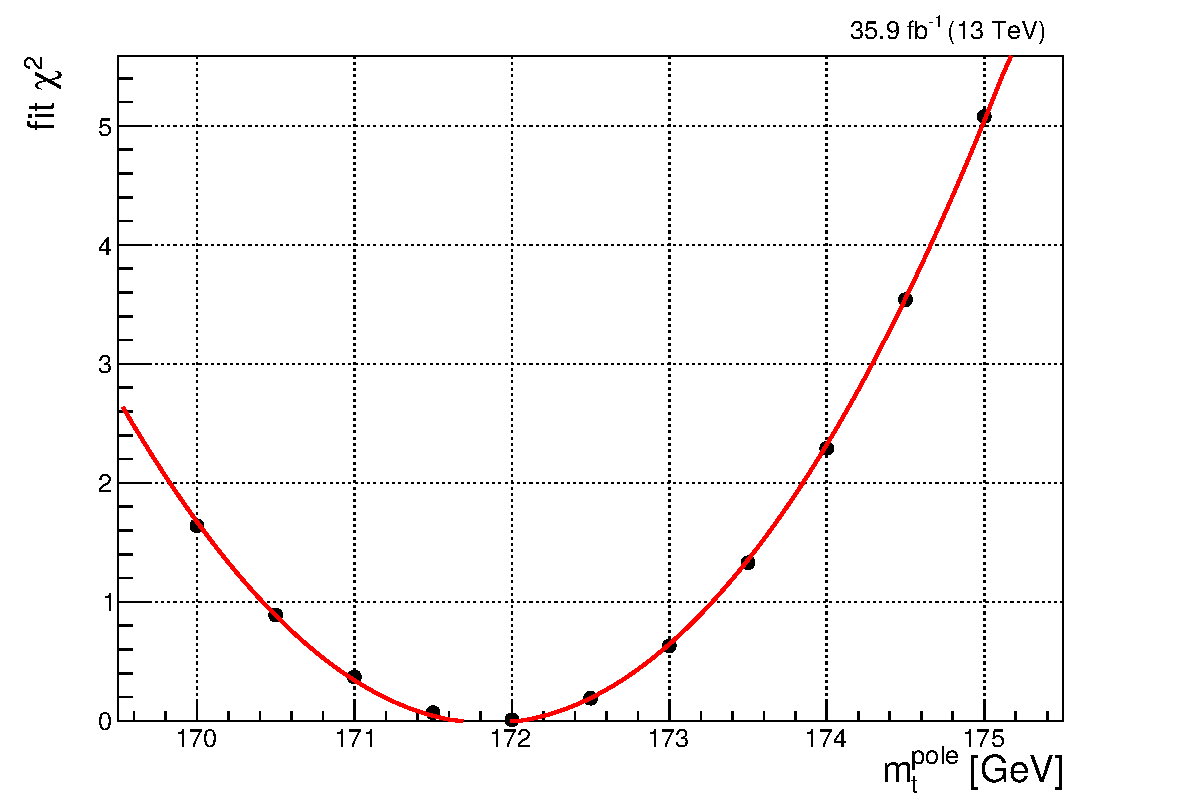
\includegraphics{Results/Figures/PoleMass}}   

\caption{The values for $\chi^2(\mtp)$ for the comparison of measured and predicted \sttbar with the nominal configuration. The red line indicates the result of the parabolic fit of the $\chi^2$ distribution. 
       \label{fig:res_polemass}}
  \end{center}
\end{figure}

\section{Addition of the semileptonic channel}
\label{sec:res_semi}

In order to asses the feasibility of a combination of the dilepton channel with the semileptonic channel, events with exactly one muon in the final state are added to the fit of the \ttbar production cross section.
In order to reduce the complexity the fit is performed for a reduced number of systematic uncertainties. Theory based uncertainties with little impact on the measurement, like the uncertainties
on color reconnection or fragmentation, are not considered. 
In order to simulate the background processes the same simulation as in the dilepton channel is used.
In general, this is should not be seen as a full measurement, but as a feasibility study.

Since no separate study on the background contributions in the single muon channel is performed, hard selection requirements are chosen:
Events are required to contain exactly one muon with $\pt > 30 \GeV$ and $\eta < 2.4$ and two b-tagged jets with $\pt > 30 \GeV$ and $\eta < 2.4$.
The muon and the jets are defined as described in Section \ref{sec:xsec_sel}.
These requirements also define the visible phase space.
Distributions of the jet \pt are chosen as observables for the template fit, in analogy to the dilepton channel, as described in Section \ref{sec:xsec_templates}.
The uncertainty on the trigger efficiency is increased to $1\%$ (before the fit), since no dedicated study on the efficiency of the single muon triggers and its uncertainty is performed.

Including these events into the fit yields the following result:

\begin{equation}
\sttbar = 835 \pm  1 ({\rm stat}) \pm  18({\rm syst}) \pm 21 ({\rm lumi}) \pb.
\end{equation}

This result is consistent with the main result in the dilepton channel.
The uncertainty is reduced mainly, due to the reduced impact of the uncertainty on the lepton efficiency. This
uncertainty is reduced from $2.1\%$ to $1.3\%$. At the same time the uncertainty on the extrapolation to the full phase space is slightly increased, since a requirement
on jets is included for the single-muon channel. Jets are in general more affected by the uncertainty on the parton shower, compared to leptons, which leads to an increased
impact of these uncertainties in the extrapolation.

The reduction in uncertainty and the agreement with the main result show that the inclusion of the semileptonic channel is a viable method to decrease the uncertainties.

The next chapter summarizes the main results of this work and offers ideas for future improvements of the analysis.

